\documentclass{article}


% if you need to pass options to natbib, use, e.g.:
%     \PassOptionsToPackage{numbers, compress}{natbib}
% before loading neurips_2024
\PassOptionsToPackage{numbers, compress}{natbib}

% ready for submission
\usepackage[final]{neurips_2024}
\usepackage{graphicx}
\usepackage{booktabs}
\usepackage{multirow}
\usepackage{amsmath}
\usepackage{enumitem}
\usepackage{algpseudocode}
\usepackage{algorithm}
\usepackage{subfig}
\usepackage{subfloat}
% to compile a preprint version, e.g., for submission to arXiv, add add the
% [preprint] option:
% \usepackage[preprint]{neurips_2024}

% to compile a camera-ready version, add the [final] option, e.g.:
%     \usepackage[final]{neurips_2024}


% to avoid loading the natbib package, add option nonatbib:
%    \usepackage[nonatbib]{neurips_2024}


\usepackage[utf8]{inputenc} % allow utf-8 input
\usepackage[T1]{fontenc}    % use 8-bit T1 fonts
\usepackage{hyperref}       % hyperlinks
\usepackage{url}            % simple URL typesetting
\usepackage{booktabs}       % professional-quality tables
\usepackage{amsfonts}       % blackboard math symbols
\usepackage{nicefrac}       % compact symbols for 1/2, etc.
\usepackage{microtype}      % microtypography
\usepackage{xcolor}         % colors
\usepackage{amsmath}
\usepackage{amssymb} 

\title{Gaussian Graph Network: Learning Efficient and Generalizable Gaussian Representations from Multi-view Images}


% The \author macro works with any number of authors. There are two commands
% used to separate the names and addresses of multiple authors: \And and \AND.
%
% Using \And between authors leaves it to LaTeX to determine where to break the
% lines. Using \AND forces a line break at that point. So, if LaTeX puts 3 of 4
% authors names on the first line, and the last on the second line, try using
% \AND instead of \And before the third author name.


% \author{%
%   Shengjun Zhang, Xin Fei, Fangfu Liu, Haixu Song, Yueqi Duan\thanks{Use footnote for providing further information
%     about author (webpage, alternative address)---\emph{not} for acknowledging
%     funding agencies.} \\
%   Department of Computer Science\\
%   Cranberry-Lemon University\\
%   Pittsburgh, PA 15213 \\
%   \texttt{hippo@cs.cranberry-lemon.edu} \\

\author{%
  Shengjun Zhang, Xin Fei, Fangfu Liu, Haixu Song, Yueqi Duan\thanks{Corresponding author.} \\
  % Department of Computer Science\\
  Tsinghua University \\
  % Pittsburgh, PA 15213 \\
  \texttt{\{zhangsj23, feix21\}@mails.tsinghua.edu.cn, duanyueqi@tsinghua.edu.cn} \\
}
\vspace{-2cm}
  % examples of more authors
  % \And
  % Coauthor \\
  % Affiliation \\
  % Address \\
  % \texttt{email} \\
  % \AND
  % Coauthor \\
  % Affiliation \\
  % Address \\
  % \texttt{email} \\
  % \And
  % Coauthor \\
  % Affiliation \\
  % Address \\
  % \texttt{email} \\
  % \And
  % Coauthor \\
  % Affiliation \\
  % Address \\
  % \texttt{email} \\

\begin{document}

\maketitle

% \newcommand\blfootnote[1]{% 
% \begingroup 
% \renewcommand\thefootnote{}\footnote{#1}% 
% \addtocounter{footnote}{-1}% 
% \endgroup 
% }
% \blfootnote{\textsuperscript{\dag}Corresponding author.}

\begin{center}
\textbf{\url{https://shengjun-zhang.github.io/GGN/}}
\end{center}

\begin{abstract}
\begin{abstract}
Fine-tuning provides an effective means to specialize pre-trained models for various downstream tasks. However, fine-tuning often incurs high memory overhead, especially for large transformer-based models, such as LLMs. While existing methods may reduce certain parts of the memory required for fine-tuning, they still require caching all intermediate activations computed in the forward pass to update weights during the backward pass. In~this work, we develop \method, a method to reduce memory usage,  specifically the memory to store intermediate activations, in the fine-tuning of transformer-based models. During the backward pass, \method approximates the gradient computation by backpropagating through just a subset of input tokens. Thus, with \method, only a subset of intermediate activations are cached during the forward pass. Also, \method can be easily combined with existing methods like LoRA, further reducing the memory cost. We evaluate our approach on pre-trained transformer models with up to billions of parameters, considering the performance on multiple downstream tasks such as text classification and question answering in a few-shot learning setup. Overall, \method achieves performance on par with full fine-tuning or representative memory-efficient fine-tuning methods,  while greatly reducing the memory footprint, especially when combined with other methods with complementary memory reduction mechanisms. We hope that our approach will facilitate the fine-tuning of large transformers,  in specializing them for specific domains or co-training them with other neural components from a larger system. Our code is available at \githubURL.
\blfootnote{\textbf{*} Equal contribution}
\end{abstract}

\end{abstract}


\section{Introduction}
Novel view synthesis is a fundamental problem in computer vision due to its widespread applications, such as virtual reality, augmented reality, robotics and so on. Remarkable progress has been made using neural implicit representations~\cite{NeRF2021ACM, LFN2021NIPS, SRN2019NIPS}, but these methods suffer from expensive time consumption in training and rendering~\cite{NSVF2020NIPS, FastNeRF2021ICCV, MipNeRF2021ICCV, KiloNeRF2021ICCV, PlenOctree2021CVPR, Plenoxels2022CVPR, EfficientNeRF2022CVPR, InstantNGP2022TOG}.
Recently, 3D Gaussian Splatting (3DGS)~\cite{3DGS2023ToG} has drawn increasing attention for explicit Gaussian representations and real-time rendering performance. Benefiting from rasterization-based rendering, 3DGS avoids dense points querying in scene space, so that it can maintain high efficiency and quality. 

Since 3DGS relies on per-subject~\cite{3DGS2023ToG} or per-frame~\cite{Dynamic3DGS2023arXiv} parameter optimization, several generalizable methods~\cite{GPSGaussian2023arXiv, MVSplat2024arXiv, pixelSplat2023arXiv, SplatterImage2023arXiv} are proposed to directly regress Gaussian parameters with feed-forward networks. 
Typically, these methods~\cite{MVSplat2024arXiv, pixelSplat2023arXiv} generate pixel-aligned Gaussians with U-Net architectures, epipolar transformers or cost volume representations for depth estimation and parameter predictions, and directly combine Gaussian groups obtained from different views as scene representations.
However, such combination of Gaussians leads to superfluous representations, where the overlapped regions are covered by similar Gaussians predicted separately from multiple images. 
While a simple solution is to delete redundant Gaussians, it ignores the connection among Gaussian groups. As illustrated in Figure~\ref{fig:teaser_1}, pixelSplat~\cite{pixelSplat2023arXiv} and MVSplat~\cite{MVSplat2024arXiv} suffer from artifacts with several times as many Gaussians as ours, while the deletion of similar Gaussians hurts rendering quality. 

To tackle the challenge, we propose Gaussian Graphs to model the relations of Gaussian groups from multiple views. 
Based on this structure, we present Gaussian Graph Network (GGN), extending conventional graph operations to Gaussian domain, so that Gaussians from different views are not independent but can learn from their neighbor groups.
Precisely, we reformulate the scalar weight of an edge to a weight matrix to depict the interactions between two Gaussian groups, and introduce a Gaussian pooling strategy to aggregate Gaussians.  
Under this definition, previous methods~\cite{pixelSplat2023arXiv, MVSplat2024arXiv} can be considered as a degraded case of Gaussian Graphs without edges. 
As shown in Figure~\ref{fig:teaser_2}, our GGN allows message passing and aggregation across Gaussians for efficiency representations. 

We conduct extensive experiments on both indoor and outdoor datasets, including RealEstate10K~\cite{RealEstate10K2018} and ACID~\cite{ACID2021ICCV}.
While the performance of previous methods declines as the number of input views increases, our method can benefit from more input views. As shown in Figure~\ref{fig:teaser_3}, our model outperforms previous methods under different input settings with higher rendering quality and fewer Gaussian representations.
Our main contributions can be summarized as follows:
\begin{itemize}[leftmargin=*]
    \item We propose Gaussian Graphs to construct the relations of different Gaussian groups, where each node is a set of pixel-aligned Gaussians from an input view.
    \item We introduce Gaussian Graph Network to process Gaussian Graphs by extending the graph operations to Gaussian domain, bridging the interaction and aggregation across Gaussian groups.
    \item Experimental results illustrate that our method can generate efficient and generalizable Gaussian representations. Our model requires fewer Gaussians and achieves better rendering quality.
\end{itemize}

\begin{figure}[t]
  \centering
      \subfloat[]{{\label{fig:teaser_1}}
      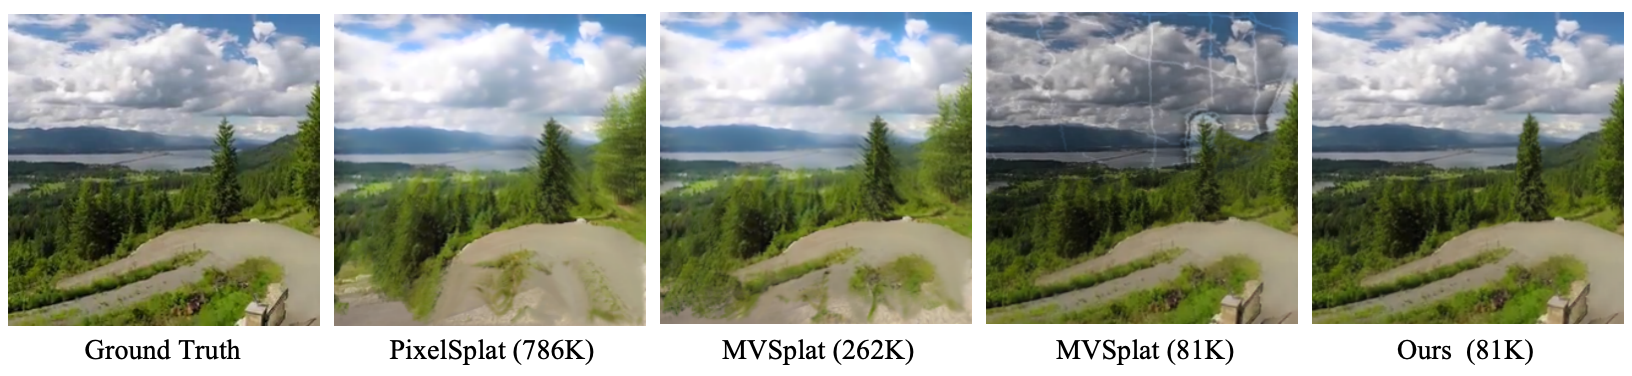
\includegraphics[height=0.22\linewidth]{fig/teaser_1.png}}
  \vspace{-0.2cm}
  \begin{minipage}[h]{0.99\linewidth}
      \centering            
      \subfloat[]{{\label{fig:teaser_2}}   
      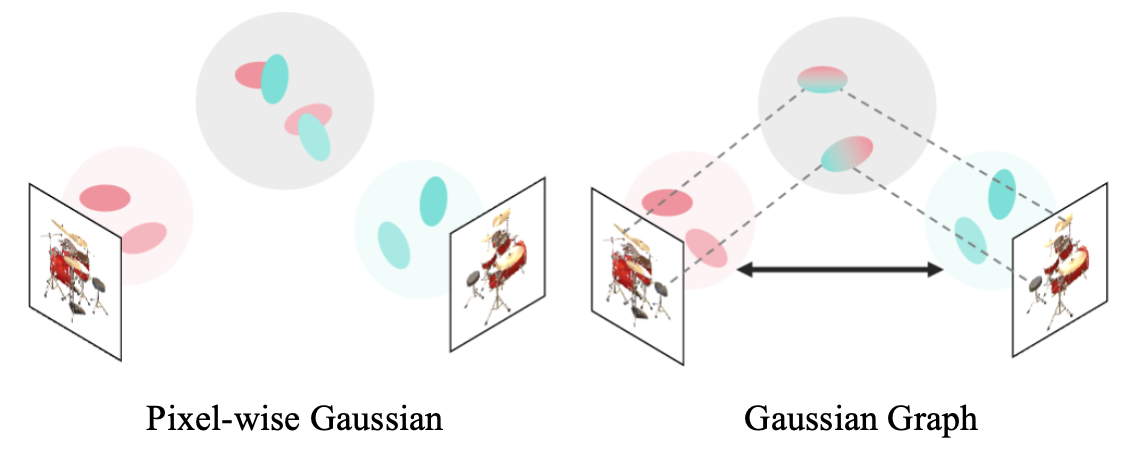
\includegraphics[height=0.26\linewidth]{fig/teaser_2.png}}
      \subfloat[]{{\label{fig:teaser_3}}
      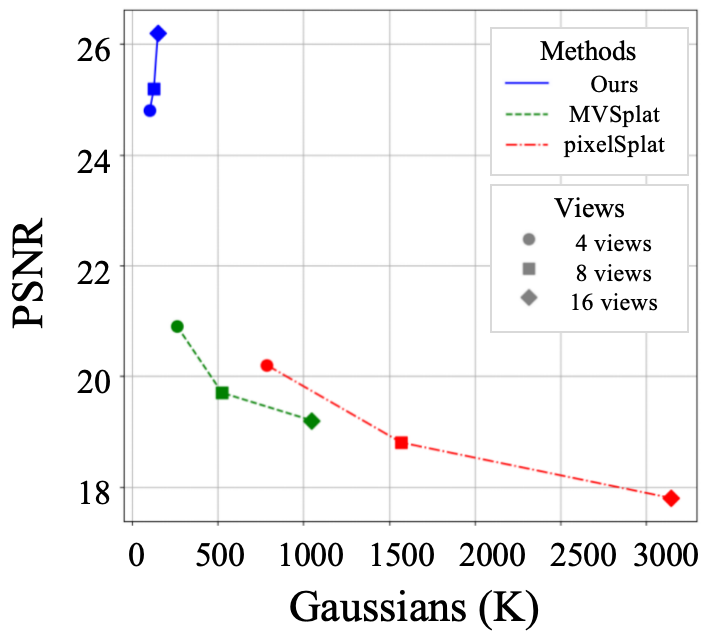
\includegraphics[height=0.26\linewidth]{fig/teaser_3.png}}
  \end{minipage}
  \caption{Comparison of previous methods and ours. (a) We visualize the rendering results of various methods and report the number of Gaussians in parentheses. (b) Previous pixel-wise methods can be considered as a degraded case of Gaussian Graphs without edges. (c) We report PSNR as well as the number of Gaussians for pixelSplat~\cite{pixelSplat2023arXiv}, MVSplat~\cite{MVSplat2024arXiv} and GNN under different input settings.}
  \label{fig:teaser}
  \vspace{-0.2cm}
\end{figure}
    


\section{Related Works}
\section{Related Work}
\label{sec:related_works}


\noindent\textbf{Panoramic scene understanding.}
Panoramic perception enables a holistic understanding of a 360{\textdegree} scene in a single shot~\cite{gao2022review,chen2024360+,dong2024panocontext,ehsanpour2022jrdb_act,jiang2024minimalist,jiang2022annular,ai2022deep}. 
Main areas include 
panoramic scene segmentation~\cite{teng2024360bev,zheng2024360sfuda++,cao2024occlusion,zheng2024semantics,yan2023panovos,jaus2021panoramic_panoptic,jaus2023panoramic_insights}, 
panoramic estimation~\cite{bai2024glpanodepth,ai2024elite360d,wang2022bifuse++,shen2022panoformer,chang2023depth_neural}, 
panoramic layout estimation~\cite{yu2023panelnet,shen2023disentangling,ling2023panoswin}, 
panoramic generation~\cite{zhou2025dreamscene360,wang2024360dvd,li2023panogen}, 
and panoramic flow estimation~\cite{shi2023panoflow,li2022deep}, \etc~\cite{park2024fully,kim2024fully,fan2024learned,han2022panoramic_activity}.
Researchers typically unfold panoramas into equirectangular projections or polyhedral projections to adapt algorithms designed for limited-FoV data~\cite{jiang2021unifuse,wang2022bifuse++,li2022deep}. 
They also apply techniques such as deformable convolutions to handle severe distortions in high-latitude regions~\cite{shi2023panoflow,zhang2024behind}.

Recently, researchers have recognized the advantages of omnidirectional images for tracking, particularly their ability to maintain continuous observation of targets without the out-of-view issues present in limited field-of-view setups.
Jiang~\etal~\cite{jiang2021500} propose a $500$FPS omnidirectional tracking system using a three-axis active vision mechanism to capture fast-moving objects in complex environments.
The 360VOT benchmark~\cite{huang2023360vot} is introduced for omnidirectional object tracking, focusing on spherical distortions and object localization challenges.
Huang~\etal~\cite{huang2024360loc} present 360Loc for omnidirectional localization that tackles cross-device challenges by generating lower-FoV query frames from 360{\textdegree} data. 
Another work by Xu~\etal~\cite{xu2024360vots} introduces an extended bounding FoV (eBFoV) representation to alleviate spherical distortions in panoramic videos.
Unlike previous methods, this work first explores extremely challenging panoramic-FoV and intense-motion panoramic tracking for mobile robots, \eg, aiming to enhance the robot’s spatiotemporal understanding of objects in its surroundings.

\noindent\textbf{Multi-object tracking.}
Object tracking primarily follows two paradigms: Tracking-By-Detection (TBD)~\cite{Chen_2024_CVPR,Du_2024_CVPR,qin2024towards,nettrack2024cvpr,huang2024deconfusetrack,lv2024diffmot,li2023ovtrack,qin2023motiontrack} and End-To-End (E2E)~\cite{ding2024adatrack,li2023end,MeMOTR,zeng2022motr}. 
Among these, TBD is currently one of the most prevalent, with frameworks following the design principles of SORT~\cite{wojke2017simple}. 
First, the detection network~\cite{yolox2021,carion2020end} is used to locate bounding boxes for objects, then the target's current position is predicted based on its historical trajectory, and the predicted results are associated with detection results~\cite{kuhn1955hungarian}. 
Many subsequent works have refined this approach: DeepSORT~\cite{li2022deep} introduced a ReID model to incorporate appearance information for association, and ByteTrack~\cite{zhang2022bytetrack} designed a confidence-based, stage-wise association strategy. 
Other methods~\cite{aharon2022bot,yi2024ucmc,du2023strongsort} introduced motion compensation modules to mitigate camera motion, and OC-SORT~\cite{cao2023observation} optimized the motion estimation module. Additionally, E2E methods have continued to evolve. 
TrackFormer~\cite{meinhardt2021trackformer} and MOTR~\cite{zeng2022motr} proposed transformer-based, End-to-End tracking approaches. 
Recent improvements~\cite{zhang2023motrv2, lv2024diffmot} have enhanced detector performance and improved data association accuracy in occlusion scenarios. 
Unlike existing methods that focus on narrow-FoV pinhole camera data with linear sensor motion, we address the challenges of MOT in panoramic-FoV scenarios, tackling issues such as geometric distortion and complex motion.

\section{Method}~\label{sec:methods}
\section{Method}
\label{sec:method}
Our approach, in line with previous methods, builds upon a pre-trained VLM, CLIP \cite{clip}. In this section, we detail the construction of our MMRL framework and the implementation specifics.

\subsection{Preliminary}
We begin by defining the notations used in our approach. CLIP comprises two encoders: an image encoder $\mathcal{V}$ and a text encoder $\mathcal{W}$.

\noindent \textbf{Image Encoding:} The image encoder $\mathcal{V}$ consists of $L$ transformer \cite{transformer} layers, denoted $\{\mathcal{V}_i\}_{i=1}^{L}$. Given an input image \( x \in \mathbb{R}^{H \times W \times 3} \), it is divided into \( M \) fixed-size patches, each projected into a patch embedding, resulting in \( E_0 \in \mathbb{R}^{M \times d_v} \), where $M$ represents the number of patches and $d_v$ the embedding dimension. The initial patch embeddings $E_0$ are combined with a learnable class token $c_0$ and positional encodings, forming the input sequence for the transformer layers. Each layer processes this sequence as
\begin{equation}
    [c_i, E_i] = \mathcal{V}_i([c_{i-1}, E_{i-1}]) \quad
    i = 1, 2, \ldots, L
    \nonumber
\end{equation}
After passing through all transformer layers, a patch projection layer, $P_v^c$, projects the output of the class token, $c_L$, into a shared V-L latent space,
\begin{equation}
    f = P_v^c(c_L)
    \nonumber
\end{equation}
where $f \in \mathbb{R}^{d}$.

\noindent \textbf{Text Encoding:} For an input text, \eg, ``A photo of a [CLASS].", it is tokenized and converted into embeddings $T_0 \in \mathbb{R}^{N \times d_t}$, where $N$ is the token length and $d_t$ the embedding dimension. Beginning-of-text (BOT) and end-of-text (EOT) tokens, denoted $b_0$ and $e_0$, mark the sequence boundaries. These token embeddings, with positional encodings, are passed through the text encoder's $L$ transformer layers, $\{\mathcal{W}_i\}_{i=1}^{L}$, as follows,
\begin{equation} 
    [b_i, T_i, e_i] = \mathcal{W}_i([b_{i-1}, T_{i-1}, e_{i-1}]) \quad i = 1, \ldots, L 
    \nonumber
\end{equation} 
After the final layer, the output of the EOT token, $e_L$, is projected into the shared V-L space using $P_t$,
\begin{equation} 
    w = P_{t}(e_{L}) \nonumber
\end{equation} 
where $w \in \mathbb{R}^{d}$.

\noindent \textbf{Classification with CLIP:} With the image feature $f$ and text features $\{w_c\}_{c=1}^C$ for $C$ classes, CLIP calculates the cosine similarity between $f$ and each $w_c$,
\begin{equation} 
    \text{sim}(f, w_c) = \frac{f \cdot w_c}{|f| |w_c|}, \nonumber 
\end{equation} 
where $|\cdot|$ represents the $L_2$ norm. Class probabilities are then computed using the softmax function,
\begin{equation} 
    p(y = c \mid f) = \frac{\exp(\text{sim}(f, w_c) / \tau)}{\sum_{i=1}^{C} \exp(\text{sim}(f, w_i) / \tau)} \nonumber 
\end{equation} 
where $\tau$ is a temperature parameter. The final predicted class is selected as the one with the highest probability score.

% The predicted class $\hat{y}$ is determined by: \begin{equation} 
%     \hat{y} = \arg\max_{c} , p(y = c \mid f). \nonumber
% \end{equation}


%-------------------------------------------------------------------------
\begin{figure*}[tb]
\setlength{\abovecaptionskip}{0.2cm}   %调整图片标题与图距离
\setlength{\belowcaptionskip}{-0.4cm}   %调整图片标题与下文距离
\centering
\setlength{\belowcaptionskip}{-0.39cm}   %调整图片标题与下文距离
  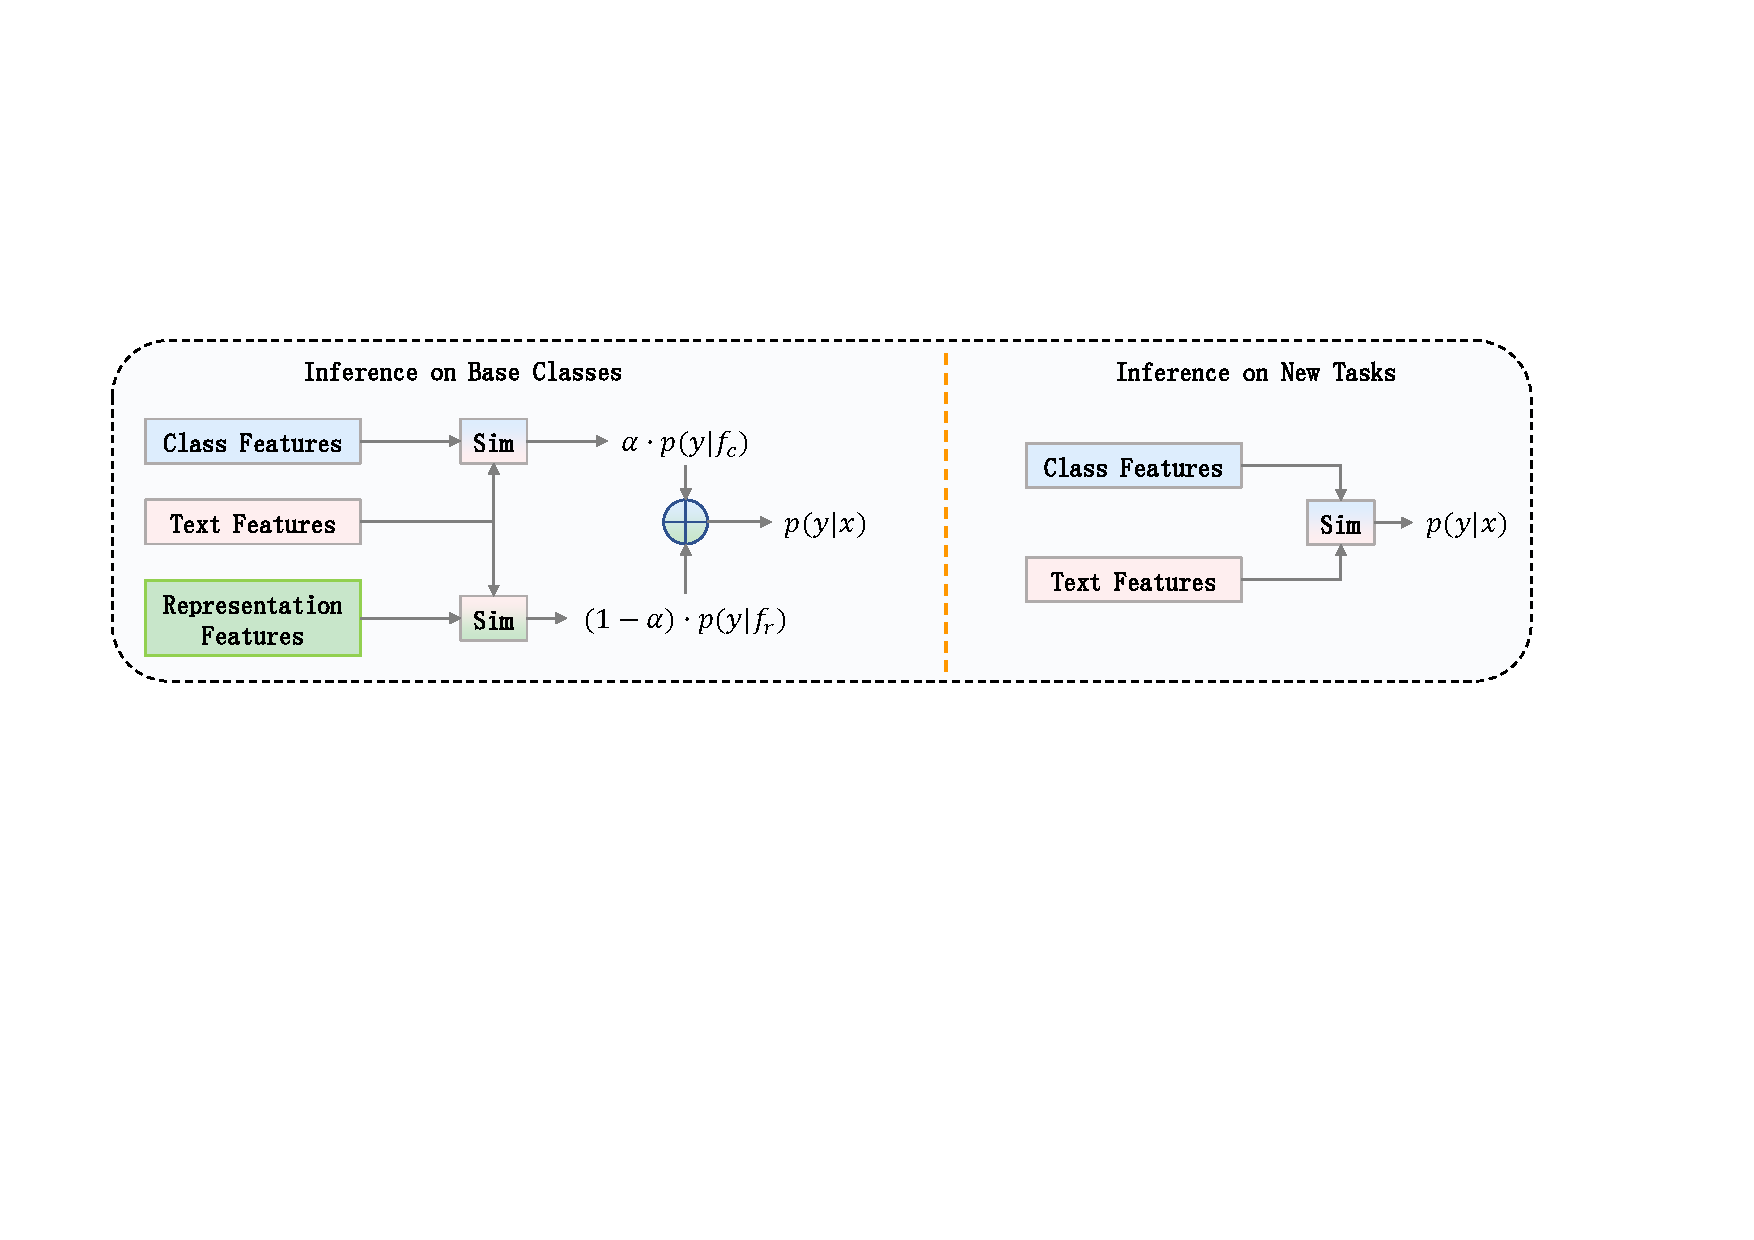
\includegraphics[width=0.7\linewidth]{fig/frame2.pdf}
  \caption{MMRL inference process, where different tasks utilize distinct features.}
  \label{framework2}
\end{figure*}
%-------------------------------------------------------------------------


\subsection{Multi-Modal Representation Learning (MMRL)} Our proposed MMRL aims to address the challenges of adapting pre-trained VLMs using few-shot data while maintaining generalization to new tasks. The training and inference frameworks of MMRL are shown in \cref{framework1} and \cref{framework2}, respectively. In the following, we describe the specifics of the methodology.


\subsubsection{Learnable Representation Space}
MMRL establishes a shared, learnable representation space $\mathcal{R}$ to facilitate multimodal interactions, initialized through sampling from a Gaussian distribution. Using a learnable mapping function $\mathcal{F}(\cdot)$, implemented as a linear layer, we project the tokens $R \in \mathbb{R}^{K \times d_r}$ in this space—where $K$ is the number of tokens and $d_r$ is the dimension of the representation space—into both visual and textual modalities,
\begin{align}
    R^v = \{R_i^v\}_{i=J-1}^{L-1} \quad & R_i^v = \mathcal{F}_i^v(R) \nonumber \\ 
    R^t = \{R_i^t\}_{i=J-1}^{L-1} \quad & R_i^t = \mathcal{F}_i^t(R) \nonumber 
\end{align}
where $R_i^v \in \mathbb{R}^{K \times d_v}$ and $R_i^t \in \mathbb{R}^{K \times d_t}$ represent the representation tokens for visual and textual modalities, respectively, in the $(i+1)$-th transformer layer. The index $J$ indicates the starting layer from which these representation tokens are integrated into the encoders.


\subsubsection{Integration into Higher Encoder Layers}
To preserve the generalized knowledge in the lower layers of the pre-trained CLIP model, the representation tokens $\mathcal{R}^v$ and $\mathcal{R}^t$ are integrated into the higher layers of the image encoder $\mathcal{V}$ and the text encoder $\mathcal{W}$, beginning from the $J$-th layer.


For the image encoder $\mathcal{V}$,
\begin{align}
    [c_i, E_i] &= \mathcal{V}_i([c_{i-1}, E_{i-1}]) \quad i = 1, \ldots, J-1 \nonumber \\  
    [c_i, \_, E_i] &= \mathcal{V}_i([c_{i-1}, R_{i-1}^v, E_{i-1}]) \quad i = J, \ldots, L - 1 \nonumber \\
    [c_i, R_i^v, E_i] &= \mathcal{V}_i([c_{i-1}, R_{i-1}^v, E_{i-1}]) \quad i = L \nonumber
\end{align}

For the text encoder $\mathcal{W}$, while previous prompt learning \cite{maple} involves replacing parts of $T_i$ to incorporate deep prompts, we retain the entire $T_i$ and insert $R_i^t$ before it, aiming to preserve the original textual information,
\begin{align}
    [b_i, T_i, e_i] &= \mathcal{W}_i([b_{i-1}, T_{i-1}, e_{i-1}]) \quad i = 1, \ldots, J-1 \nonumber \\  
    [b_i, \_, T_i, e_i] &= \mathcal{W}_i([b_{i-1}, R_{i-1}^t, T_{i-1}, e_{i-1}]) \nonumber \\
    &\hspace{4cm} i = J, \ldots, L-1 \nonumber \\
    [b_i, R_i^t, T_i, e_i] &= \mathcal{W}_i([b_{i-1}, R_{i-1}^t, T_{i-1}, e_{i-1}]) \quad i = L \nonumber
\end{align}
Note that due to the autoregressive nature of the text encoder, we adjust the attention mask matrix to accommodate the increased embedding length.


\subsubsection{Representation Learning}
Representation learning is designed to leverage representation tokens for dataset-specific adaptation, while the class token preserves the pre-trained knowledge of the original CLIP. Through a set of strategies aimed at retaining generalization during both training and inference, MMRL enables flexible inference for different tasks, as detailed below.


\begin{itemize} 

\item \textbf{Training Phase:} We optimize the features of both the representation tokens and the original class token, with the primary focus on representation features to preserve pre-trained knowledge. Specifically, the projection layer for the representation tokens is trainable, while that for the class token remains fixed. For the image encoder $\mathcal{V}$, after passing through $L$ transformer layers, we obtain the output $c_L \in \mathbb{R}^{d_v}$ for the class token and $R_L^v \in \mathbb{R}^{K \times d_v}$ for the $K$ representation tokens. The final output of the representation tokens, $r_L$, is derived by averaging across the $K$ tokens,
\begin{equation}
    r_L = \text{Mean}(R_L^v) \nonumber
\end{equation}
where $r_L \in \mathbb{R}^{d_v}$. We then apply the patch projection layers to map the outputs of both the class and representation tokens into the common V-L latent space, yielding the class features $f_c$ and representation features $f_r$.
\begin{equation}
    f_c = P_v^c(c_L) \quad f_r = P_v^r(r_L) \nonumber
\end{equation}
Here, $P_v^c$ is the original, frozen patch projection layer of CLIP for class features, while $P_v^r$ for representation features is trainable.

For the text encoder $\mathcal{W}$, following the sequential nature of text, we map the EOT token $e_L$—as in the original CLIP model—after processing through $L$ transformer layers into the common V-L space, yielding the text features.
\begin{equation} 
    w = P_{t}(e_{L}) \nonumber
\end{equation}
With the image features $f_c$, $f_r$, and the text classifiers $\{w_c\}_{c=1}^C$ for $C$ classes, we apply cross-entropy loss to separately optimize the class and representation features,
\begin{align}
\setlength\abovedisplayskip{3pt}
\setlength\belowdisplayskip{3pt}
    \mathcal{L}_{ce}^c &= -\sum_c^C y_c \log p(y = c \mid f_c) \nonumber \\
    \mathcal{L}_{ce}^r &= -\sum_c^C y_c \log p(y = c \mid f_r) \nonumber
\end{align}
where $y_c = 1$ if the image $x$ belongs to class $c$, and $y_c = 0$ otherwise. To further preserve the generalization of class features, we maximize the cosine similarity between $(f_c, w)$ and the frozen CLIP features $(f_0, w_0)$, explicitly guiding the training trajectory,
\begin{equation}
    \mathcal{L}_{cos}^v = 1 - \frac{f_c \cdot f_0}{|f_c| |f_0|} \quad \mathcal{L}_{cos}^t = 1 - \frac{1}{C}\sum_c^C \frac{w^c \cdot w_0^c}{|w^c| |w_0^c|}, \nonumber
\end{equation}
The final MMRL loss function is
\begin{equation}
    \mathcal{L}_{MMRL} = \alpha \mathcal{L}_{ce}^c + (1 - \alpha) \mathcal{L}_{ce}^r + \lambda (\mathcal{L}_{cos}^v + \mathcal{L}_{cos}^t)  \nonumber
\end{equation}
where $\alpha$ controls the balance between the features, and $\lambda$ is the penalty coefficient.

\item \textbf{Testing on Base Classes:} 
For in-distribution classes seen during training, we combine the dataset-specific representation features with the class features that preserve generalizability. The probability of an in-distribution test sample $x$ belonging to the $c$-th class is
\begin{equation}
    p(y = c \mid x) = \alpha \cdot p(y = c \mid f_c) + (1-\alpha) \cdot p(y = c \mid f_r) \nonumber
\end{equation}
where $f_c$ and $f_r$ are features extracted from the class token and representation tokens, respectively.

\item  \textbf{Testing on Novel Classes:}
For classes unseen during training or for new datasets, we rely solely on the class tokens, which retain generalized knowledge.
\begin{equation}
    p(y = c \mid x) = p(y = c \mid f_c) \nonumber
\end{equation}
\end{itemize}



% Then the predicted class $\hat{y}$ is determined by, 
% \begin{equation} 
%     \hat{y} = \arg\max_{c} , p(y = c \mid x). \nonumber
% \end{equation}



\begin{table*}[t]
\centering
\setlength{\abovecaptionskip}{0.15cm}   %调整表格标题与表格距离
\caption{Comparison of MMRL with previous state-of-the-art methods on base-to-novel generalization across 11 datasets. Bold values indicate the best results. MMRL consistently enhances base class performance without compromising generalization.}
\label{base_to_novel}
\renewcommand\arraystretch{1.06}
\setlength{\tabcolsep}{2.87mm}{
\resizebox{0.85\textwidth}{!}{
    \begin{tabular}{@{}r|ccc|ccc|ccc|ccc@{}}
    \toprule
    \multirow{2}{*}{Method} &
      \multicolumn{3}{c|}{Average} &
      \multicolumn{3}{c|}{ImageNet} &
      \multicolumn{3}{c|}{Caltech101} &
      \multicolumn{3}{c}{OxfordPets} \\
     &
      Base &
      Novel &
      HM &
      Base &
      Novel &
      HM &
      Base &
      Novel &
      HM &
      Base &
      Novel &
      HM \\ \midrule
    $\text{CLIP}_{\text{ (ICML2021)}}$ &
      69.34 &
      74.22 &
      71.70 &
      72.43 &
      68.14 &
      70.22 &
      96.84 &
      94.00 &
      95.40 &
      91.17 &
      97.26 &
      94.12 \\
    $\text{CoOp}_{\text{ (IJCV2022)}}$ &
      82.69 &
      63.22 &
      71.66 &
      76.47 &
      67.88 &
      71.92 &
      98.00 &
      89.81 &
      93.73 &
      93.67 &
      95.29 &
      94.47 \\
    $\text{CoOpOp}_{\text{ (CVPR2022)}}$ &
      80.47 &
      71.69 &
      75.83 &
      75.98 &
      70.43 &
      73.10 &
      97.96 &
      93.81 &
      95.84 &
      95.20 &
      97.69 &
      96.43 \\
    $\text{ProDA}_{\text{ (CVPR2022)}}$ &
      81.56 &
      72.30 &
      76.65 &
      75.40 &
      70.23 &
      72.72 &
      98.27 &
      93.23 &
      95.68 &
      95.43 &
      97.83 &
      96.62 \\
    $\text{KgCoOp}_{\text{ (CVPR2023)}}$ &
      80.73 &
      73.60 &
      77.00 &
      75.83 &
      69.96 &
      72.78 &
      97.72 &
      94.39 &
      96.03 &
      94.65 &
      97.76 &
      96.18 \\
    $\text{MaPLe}_{\text{ (CVPR2023)}}$ &
      82.28 &
      75.14 &
      78.55 &
      76.66 &
      70.54 &
      73.47 &
      97.74 &
      94.36 &
      96.02 &
      95.43 &
      97.76 &
      96.58 \\
    $\text{PromptSRC}_{\text{ (ICCV2023)}}$ &
      84.26 &
      76.10 &
      79.97 &
      77.60 &
      70.73 &
      74.01 &
      98.10 &
      94.03 &
      96.02 &
      95.33 &
      97.30 &
      96.30 \\
    $\text{ProVP}_{\text{ (IJCV2024)}}$ &
      85.20 &
      73.22 &
      78.76 &
      75.82 &
      69.21 &
      72.36 &
      98.92 &
      94.21 &
      96.51 &
      95.87 &
      97.65 &
      \textbf{96.75} \\
    $\text{MetaPrompt}_{\text{ (TIP2024)}}$ &
      83.65 &
      75.48 &
      79.09 &
      77.52 &
      70.83 &
      74.02 &
      98.13 &
      94.58 &
      96.32 &
      95.53 &
      97.00 &
      96.26 \\
    $\text{TCP}_{\text{ (CVPR2024)}}$ &
      84.13 &
      75.36 &
      79.51 &
      77.27 &
      69.87 &
      73.38 &
      98.23 &
      \textbf{94.67} &
      96.42 &
      94.67 &
      97.20 &
      95.92 \\
    $\text{MMA}_{\text{ (CVPR2024)}}$ &
      83.20 &
      76.80 &
      79.87 &
      77.31 &
      71.00 &
      74.02 &
      98.40 &
      94.00 &
      96.15 &
      95.40 &
      \textbf{98.07} &
      96.72 \\ \midrule
    $\text{MMRL}_{\text{ (Ours)}}$ &
      \textbf{85.68} &
      \textbf{77.16} &
      \textbf{81.20} &
      \textbf{77.90} &
      \textbf{71.30} &
      \textbf{74.45} &
      \textbf{98.97} &
      94.50 &
      \textbf{96.68} &
      \textbf{95.90} &
      97.60 &
      96.74 \\ \midrule \midrule
    \multirow{2}{*}{Method} &
      \multicolumn{3}{c|}{StanfordCars} &
      \multicolumn{3}{c|}{Flowers102} &
      \multicolumn{3}{c|}{Food101} &
      \multicolumn{3}{c}{FGVCAircraft} \\
     &
      Base &
      Novel &
      HM &
      Base &
      Novel &
      HM &
      Base &
      Novel &
      HM &
      Base &
      Novel &
      HM \\ \midrule
    $\text{CLIP}_{\text{ (ICML2021)}}$ &
      63.37 &
      74.89 &
      68.65 &
      72.08 &
      77.80 &
      74.83 &
      90.10 &
      91.22 &
      90.66 &
      27.19 &
      36.29 &
      31.09 \\
    $\text{CoOp}_{\text{ (IJCV2022)}}$ &
      78.12 &
      60.40 &
      68.13 &
      97.60 &
      59.67 &
      74.06 &
      88.33 &
      82.26 &
      85.19 &
      40.44 &
      22.30 &
      28.75 \\
    $\text{CoOpOp}_{\text{ (CVPR2022)}}$ &
      70.49 &
      73.59 &
      72.01 &
      94.87 &
      71.75 &
      81.71 &
      90.70 &
      91.29 &
      90.99 &
      33.41 &
      23.71 &
      27.74 \\
    $\text{ProDA}_{\text{ (CVPR2022)}}$ &
      74.70 &
      71.20 &
      72.91 &
      97.70 &
      68.68 &
      80.66 &
      90.30 &
      88.57 &
      89.43 &
      36.90 &
      34.13 &
      35.46 \\
    $\text{KgCoOp}_{\text{ (CVPR2023)}}$ &
      71.76 &
      75.04 &
      73.36 &
      95.00 &
      74.73 &
      83.65 &
      90.50 &
      91.70 &
      91.09 &
      36.21 &
      33.55 &
      34.83 \\
    $\text{MaPLe}_{\text{ (CVPR2023)}}$ &
      72.94 &
      74.00 &
      73.47 &
      95.92 &
      72.46 &
      82.56 &
      90.71 &
      \textbf{92.05} &
      \textbf{91.38} &
      37.44 &
      35.61 &
      36.50 \\
    $\text{PromptSRC}_{\text{ (ICCV2023)}}$ &
      78.27 &
      74.97 &
      76.58 &
      98.07 &
      76.50 &
      85.95 &
      90.67 &
      91.53 &
      91.10 &
      42.73 &
      \textbf{37.87} &
      40.15 \\
    $\text{ProVP}_{\text{ (IJCV2024)}}$ &
      80.43 &
      67.96 &
      73.67 &
      98.42 &
      72.06 &
      83.20 &
      90.32 &
      90.91 &
      90.61 &
      \textbf{47.08} &
      29.87 &
      36.55 \\
    $\text{MetaPrompt}_{\text{ (TIP2024)}}$ &
      76.34 &
      75.01 &
      75.48 &
      97.66 &
      74.49 &
      84.52 &
      \textbf{90.74} &
      91.85 &
      91.29 &
      40.14 &
      36.51 &
      38.24 \\
    $\text{TCP}_{\text{ (CVPR2024)}}$ &
      80.80 &
      74.13 &
      77.32 &
      97.73 &
      75.57 &
      85.23 &
      90.57 &
      91.37 &
      90.97 &
      41.97 &
      34.43 &
      37.83 \\
    $\text{MMA}_{\text{ (CVPR2024)}}$ &
      78.50 &
      73.10 &
      75.70 &
      97.77 &
      75.93 &
      85.48 &
      90.13 &
      91.30 &
      90.71 &
      40.57 &
      36.33 &
      38.33 \\ \midrule
    $\text{MMRL}_{\text{ (Ours)}}$ &
      \textbf{81.30} &
      \textbf{75.07} &
      \textbf{78.06} &
      \textbf{98.97} &
      \textbf{77.27} &
      \textbf{86.78} &
      90.57 &
      91.50 &
      91.03 &
      46.30 &
      37.03 &
      \textbf{41.15} \\ \midrule \midrule
    \multirow{2}{*}{Method} &
      \multicolumn{3}{c|}{SUN397} &
      \multicolumn{3}{c|}{DTD} &
      \multicolumn{3}{c|}{EuroSAT} &
      \multicolumn{3}{c}{UCF101} \\
     &
      Base &
      Novel &
      HM &
      Base &
      Novel &
      HM &
      Base &
      Novel &
      HM &
      Base &
      Novel &
      HM \\ \midrule
    $\text{CLIP}_{\text{ (ICML2021)}}$ &
      69.36 &
      75.35 &
      72.23 &
      53.24 &
      59.90 &
      56.37 &
      56.48 &
      64.05 &
      60.03 &
      70.53 &
      77.50 &
      73.85 \\
    $\text{CoOp}_{\text{ (IJCV2022)}}$ &
      80.60 &
      65.89 &
      72.51 &
      79.44 &
      41.18 &
      54.24 &
      92.19 &
      54.74 &
      68.69 &
      84.69 &
      56.05 &
      67.46 \\
    $\text{CoOpOp}_{\text{ (CVPR2022)}}$ &
      79.74 &
      76.86 &
      78.27 &
      77.01 &
      56.00 &
      64.85 &
      87.49 &
      60.04 &
      71.21 &
      82.33 &
      73.45 &
      77.64 \\
    $\text{ProDA}_{\text{ (CVPR2022)}}$ &
      78.67 &
      76.93 &
      77.79 &
      80.67 &
      56.48 &
      66.44 &
      83.90 &
      66.00 &
      73.88 &
      85.23 &
      71.97 &
      78.04 \\
    $\text{KgCoOp}_{\text{ (CVPR2023)}}$ &
      80.29 &
      76.53 &
      78.36 &
      77.55 &
      54.99 &
      64.35 &
      85.64 &
      64.34 &
      73.48 &
      82.89 &
      76.67 &
      79.65 \\
    $\text{MaPLe}_{\text{ (CVPR2023)}}$ &
      80.82 &
      78.70 &
      79.75 &
      80.36 &
      59.18 &
      68.16 &
      94.07 &
      73.23 &
      82.35 &
      83.00 &
      78.66 &
      80.77 \\
    $\text{PromptSRC}_{\text{ (ICCV2023)}}$ &
      82.67 &
      78.47 &
      80.52 &
      83.37 &
      62.97 &
      71.75 &
      92.90 &
      73.90 &
      82.32 &
      87.10 &
      78.80 &
      82.74 \\
    $\text{ProVP}_{\text{ (IJCV2024)}}$ &
      80.67 &
      76.11 &
      78.32 &
      83.95 &
      59.06 &
      69.34 &
      \textbf{97.12} &
      72.91 &
      83.29 &
      \textbf{88.56} &
      75.55 &
      81.54 \\
    $\text{MetaPrompt}_{\text{ (TIP2024)}}$ &
      82.26 &
      79.04 &
      80.62 &
      83.10 &
      58.05 &
      68.35 &
      93.53 &
      75.21 &
      83.38 &
      85.33 &
      77.72 &
      81.35 \\
    $\text{TCP}_{\text{ (CVPR2024)}}$ &
      82.63 &
      78.20 &
      80.35 &
      82.77 &
      58.07 &
      68.25 &
      91.63 &
      74.73 &
      82.32 &
      87.13 &
      \textbf{80.77} &
      83.83 \\
    $\text{MMA}_{\text{ (CVPR2024)}}$ &
      82.27 &
      78.57 &
      80.38 &
      83.20 &
      \textbf{65.63} &
      73.38 &
      85.46 &
      \textbf{82.34} &
      83.87 &
      86.23 &
      80.03 &
      82.20 \\ \midrule
    $\text{MMRL}_{\text{ (Ours)}}$ &
      \textbf{83.20} &
      \textbf{79.30} &
      \textbf{81.20} &
      \textbf{85.67} &
      65.00 &
      \textbf{73.82} &
      95.60 &
      80.17 &
      \textbf{87.21} &
      88.10 &
      80.07 &
      \textbf{83.89} \\ \bottomrule
    \end{tabular}
            }
}
\vspace{-0.3cm}
\end{table*}






\section{Experiments}~\label{sec:experiments}


\begin{table*}[ht]
\centering
\small
\renewcommand{\arraystretch}{0.95}
\renewcommand\tabcolsep{4pt}
\begin{tabular}{cc|c|c|c|c|ccc}
\hline 
\multicolumn{2}{c|}{Dataset} & Model & Venue & Base & Method & mAP$\uparrow$ & Rank-1$\uparrow$ & $\text{ID}^2$$\downarrow$ \\ \hline
% \multicolumn{2}{c|}{} & & & & ori & 3.34 & 11.4 & 0.5135 \\ \cline{6-9} 
% \multicolumn{2}{c|}{} & \multirow{-2}{*}{TransReID\cite{he2021transreid}(w/o training)} & & & +ours & 52.81\scriptsize{(+49.47)} & 78.92\scriptsize{(+67.52)} & 0.2158 \\ \cline{3-3} \cline{6-9} 
\multicolumn{2}{c|}{} & & & & official & 79.88 & 91.48 & 0.2193 \\ \cline{6-9} 
\multicolumn{2}{c|}{} & \multirow{-2}{*}{TransReID\cite{he2021transreid}(w/o camid)} & & & +ours & 90.39\scriptsize{(+10.51)} & 94.74\scriptsize{(+3.26)} & 0.1357 \\ \cline{3-3} \cline{6-9} 
\multicolumn{2}{c|}{} & & & & official & 89 & 95.1 & 0.2759 \\ \cline{6-9} 
\multicolumn{2}{c|}{} & \multirow{-2}{*}{TransReID\cite{he2021transreid}(w/ camid)} & \multirow{-4}{*}{ICCV21} & \multirow{-4}{*}{ViT} & +ours & 93.01\scriptsize{(+4.01)} & 95.52\scriptsize{(+0.42)} & 0.1967 \\ \cline{3-9} 
\multicolumn{2}{c|}{} & & & & official & 89.7 & 95.4 & 0.0993 \\ \cline{6-9} 
\multicolumn{2}{c|}{} & & & \multirow{-2}{*}{ViT} & +ours & 94\scriptsize{(+4.3)} & 96.4\scriptsize{(+1.0)} & 0.0624 \\ \cline{5-9} 
\multicolumn{2}{c|}{} & & & & official & 89.8 & 95.7 & 0.0877 \\ \cline{6-9} 
\multicolumn{2}{c|}{\multirow{-8}{*}{Market1501}} & \multirow{-4}{*}{CLIP-ReID\cite{li2023clip}} & \multirow{-4}{*}{AAAI23} & \multirow{-2}{*}{CNN} & \cellcolor{gray!20}+ours & \cellcolor{gray!20}94.9\scriptsize{(+5.1)} & \cellcolor{gray!20}97.3\scriptsize{(+1.6)} & \cellcolor{gray!20}0.053 \\ \hline
\multicolumn{2}{c|}{} & & & & official & 79.05 & 85.4 & 0.3124 \\ \cline{6-9} 
\multicolumn{2}{c|}{} & \multirow{-2}{*}{KPR\cite{somers2025keypoint}} & \multirow{-2}{*}{ECCV24} & \multirow{-2}{*}{ViT} & \cellcolor{gray!20}+ours & \cellcolor{gray!20}89.34\scriptsize{(+10.29)} & \cellcolor{gray!20}91\scriptsize{(+5.6)} & \cellcolor{gray!20}0.1434 \\ \cline{3-9} 
\multicolumn{2}{c|}{} & & & & official & 70.41 & 77.2 & 0.377 \\ \cline{6-9} 
\multicolumn{2}{c|}{\multirow{-4}{*}{Occluded-ReID}} & \multirow{-2}{*}{BPBReID\cite{somers2023body}} & \multirow{-2}{*}{WACV23} & \multirow{-2}{*}{ViT} & +ours & 86.05\scriptsize{(+15.64)} & 89.1\scriptsize{(+11.9)} & 0.1504 \\ \hline
\multicolumn{1}{c|}{} & & & & & official & 71.81 & 75.29 & 0.4817 \\ \cline{6-9} 
\multicolumn{1}{c|}{} & \multirow{-2}{*}{All} & & & & \cellcolor{gray!20}+ours & \cellcolor{gray!20}76.44\scriptsize{(+4.63)} & \cellcolor{gray!20}79.33\scriptsize{(+4.04)} & \cellcolor{gray!20}0.4072 \\ \cline{2-2} \cline{6-9} 
\multicolumn{1}{c|}{} & & & & & official & 84.6 & 81.59 & 0.4424 \\ \cline{6-9} 
\multicolumn{1}{c|}{} & \multirow{-2}{*}{Indoor} & \multirow{-4}{*}{SAAI\cite{fang2023visible}} & \multirow{-4}{*}{ICCV23} & \multirow{-4}{*}{CNN} & \cellcolor{gray!20}+ours & \cellcolor{gray!20}86.83\scriptsize{(+2.23)} & \cellcolor{gray!20}84.2\scriptsize{(+2.61)} & \cellcolor{gray!20}0.3694 \\ \cline{2-9} 
\multicolumn{1}{c|}{} & & & & & official & 66.13 & 67.7 & 0.4308 \\ \cline{6-9} 
\multicolumn{1}{c|}{} & \multirow{-2}{*}{All} & & & & +ours & 75.43\scriptsize{(+9.3)} & 74.81\scriptsize{(+7.11)} & 0.3133 \\ \cline{2-2} \cline{6-9} 
\multicolumn{1}{c|}{} & & & & & official & 77.81 & 72.95 & 0.4046 \\ \cline{6-9} 
\multicolumn{1}{c|}{\multirow{-8}{*}{SYSU-MM01}} & \multirow{-2}{*}{Indoor} & \multirow{-4}{*}{PMT\cite{lu2023learning}} & \multirow{-4}{*}{AAAI23} & \multirow{-4}{*}{ViT} & +ours & 84.29\scriptsize{(+6.48)} & 80.29\scriptsize{(+7.34)} & 0.2995 \\ \hline
\end{tabular}

\caption{Improvements with our method on different SOTA models with both ViT and CNN backbone on Market1501, SYSU-MM01, and Occluded-ReID datasets. The data under \colorbox{gray!20}{grey} is the new SOTA with our methods of that dataset.}
\label{tab:sota}
\end{table*}


\begin{table*}[ht]
\centering
\small
\renewcommand{\arraystretch}{1.0}
\renewcommand\tabcolsep{4pt}
\begin{minipage}{0.32\textwidth}
\centering
\begin{tabular}{c|ccc}
\hline
\textbf{Methods} & mAP$\uparrow$ & Rank-1$\uparrow$ & $\text{ID}^2$$\downarrow$ \\ \hline
Base & 79.88 & 91.48 & 0.2193 \\
+NFC & 83.92 & 91.83 & 0.1824 \\
+IPG & 88.02 & 94.77 & 0.1553 \\
\rowcolor{gray!20}
+NFC+IPG & 90.39 & 94.74 & 0.1357 \\
\hline
\end{tabular}
\caption{Ablation study on effects of feature centralization through Identity-Guided Pedestrian Generation (IPG) and Neighbor Feature Centralization (NFC).}
\label{tab:ablation_fe_pg}
\end{minipage}
\hfill
\begin{minipage}{0.32\textwidth}
\centering
\begin{tabular}{cc|cc}
\hline
$\text{Gallery}^\text{NFC}$ & $\text{Query}^\text{NFC}$  & mAP$\uparrow$ & Rank-1$\uparrow$ \\ \hline
 \ding{55} & \ding{55}   & 79.88&	91.48  \\
 \ding{51} & \ding{55}    & 81.70 & 92.04  \\
\ding{55} & \ding{51}    & 82.76 & 91.69  \\
\rowcolor{gray!20}
\ding{51} & \ding{51}    & 83.92 & 91.83 \\ 
\hline
\end{tabular}
\caption{Ablation study of Neighbor Feature Centralization (NFC) Algorithm on Market1501 dataset. We test on the gallery and query set respectively.}
\label{tab:as_fe}
\end{minipage}
\hfill
\begin{minipage}{0.32\textwidth}
\centering
\begin{tabular}{cc|cc}
\hline
% \multicolumn{2}{c|}{\textbf{Methods}}& \multicolumn{4}{c}{Metrics}  \\ \hline
$\text{Gallery}^\text{IPG}$ & $\text{Query}^\text{IPG}$  & mAP$\uparrow$ & Rank-1$\uparrow$ \\ \hline
\ding{55} & \ding{55}   & 79.88&	91.48  \\
% \ding{51} & \ding{55}    &  84.06 &91.48 \\
% \ding{55} & \ding{51}    & 81.01 &91.03  \\
% \rowcolor{gray!20}
% \ding{51} & \ding{51}    & 87.38& 94.63 \\ 
 \ding{51} & \ding{55}    & 84.65&	92.07  \\
\ding{55} & \ding{51}    & 82.18	&92.40  \\
\rowcolor{gray!20}
\ding{51} & \ding{51}    &88.02&	94.77 \\ 
\hline
\end{tabular}
\caption{Ablation study of Feature ID-Centralizing with Pedestrian Generation (IPG) on Market1501. We test on gallery and query set respectively.}
\label{tab:as_gen}
\end{minipage}
\end{table*}


\begin{table}
\small
    \centering
    \renewcommand{\arraystretch}{1}
    \renewcommand\tabcolsep{6pt}
    \begin{tabular}{c|ccccc}
        \hline
        \textbf{Method} & mAP$\uparrow$ & R1$\uparrow$ & R5$\uparrow$ & R10$\uparrow$ & $\text{ID}^2$$\downarrow$ \\ \hline
        w/o training & 3.34 & 11.4 & 21.88 & 28 & 0.5135 \\
        \rowcolor{gray!20}
        +IPG & 52.81 & 78.92 & 91.21 & 94.27 & 0.2158 \\
        \rowcolor{gray!20}
        +IPG+NFC & 57.27 & 82.39 & 90.17 & 92.81 & 0.1890 \\ \hline
    \end{tabular}
    \caption{ReID performance on Market1501 with only ImageNet pre-trained weights without ReID training. The distribution visualized in Fig.\ref{fig:noise_tsne}.}
    \label{tab:notraining}
\end{table}
\begin{figure}[H]
\centering
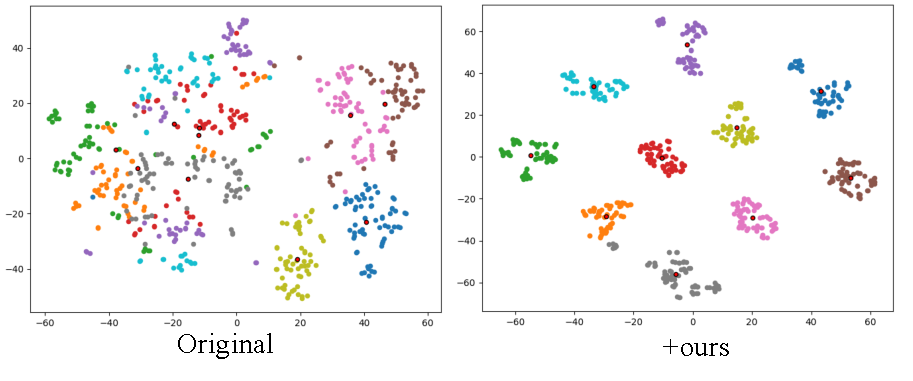
\includegraphics[width=0.95\linewidth]{figs/pdf/noise_tsne.pdf}
\caption{t-SNE visualization of 10 IDs feature distribution with and without our method on ImageNet pre-trained weights.}
\label{fig:noise_tsne}
\end{figure}


\section{Experiments}
\subsection{Implementation Details}

\textbf{Data Cleaning.}
Training an effective generative model requires high-quality data support. In current ReID (Person Re-Identification) datasets, there are many low-quality images, and removing them can help reduce interference to the model. In our experiments, we found two main issues that need to be addressed:\textbf{Extremely Low-quality Images}: The dataset contains images with such low resolution that even the human eye cannot recognize them as a "person". \textbf{Pose Estimation Failures}: The pose estimation model inevitably fails to detect pedestrian poses in some images.

Utilizing the feature distribution mentioned in Section\ref{Feature Distribution}, we can solve the issues and get the reference image set $S_i^{\text{ref}}$ and target image set $S^{\text{trg}}_i$ of identity $i$.
The cleansing process is detailed in \textbf{Supplementary}. 
\\
\textbf{Identity-guided Pedestrian Generation model details}
For the reference UNet and denoising UNet, we use the pretrained weights of Stable Diffusion v1.5\cite{rombach2022high}. The VAE encoder and decoder initialized with official weights\cite{kingma2013auto} and froze. For the ReID model, we use pre-trained TransReID\cite{he2021transreid} without cameras on Market1501 and freeze. 

The training data collected from training set of Market1501\cite{zheng2015scalable},  Mars\cite{zheng2016mars}, MSMT17\cite{wei2018person} and SYSU-MM01\cite{wu2017rgb}, with a total of 1946 different IDs. The model was trained for 80,000 iterations on one L20(48G) GPU with batch size of 4, which costs about 20 hours, and optimized by Adam\cite{kingma2014adam} with a learning rate of 1e-5 and weight decay of 0.01. All images are resized to 512×256. We applied random flip and random erasing\cite{zhong2020random} data augmentation only on reference images.

According to Section\ref{standard pose}, we selected 8 poses on the market1501 dataset as the representative poses. Each image in test set generates 8 images with these representative poses. The generation uses DDIM with 20 steps, classifier-free guidance with a scale of 3.5, and generator seed of 42.
\\
\textbf{ReID test settings}
Test models are loaded with official open-source pre-trained models for testing. In addition, considering the generated images do not have camera IDs, so for feature consistency, we test without camera IDs (e.g. TransReID). To validate the effectiveness of our proposed method, image flip (Section\ref{flip}) trick is \textbf{NOT} applied in our experiments. On Market1501, set \(\eta=2\), and \(k_1=k_2=2\). On Occluded REID, set \(\eta=1\), and \(k_1=k_2=1\). On SYSU-MM01, set \(\eta=1/4\), and \(k_1=k_2=2\). The parameters analysis detailed in \textbf{Supplementary}.



\subsection{Improvements on State-of-the-art Methods}
To verify the exceptional feature enhancement performance of our framework, we selected state-of-the-art models of three ReID tasks, divided into CNN and ViT-based models, to demonstrate that our theory can apply to any model and various ReID tasks. As shown in Table.\ref{tab:sota}, we achieved excellent enhancements on different models.

It is worth mentioning that we help models achieve new \textbf{SOTAs} without re-rank on 3 benchmarks:
\begin{itemize}
    \item[$\bullet$] \textbf{CNN-base CLIP-ReID on market1501: }
    
    \setlength{\parindent}{1em} mAP 94.9\%, Rank-1 97.3\%. 
    \item[$\bullet$] \textbf{KPR on Occluded-ReID: }

    \setlength{\parindent}{1em} mAP 89.34\%, Rank-1 91\%
    
    \item[$\bullet$] \textbf{SAAI on SYSU-MM01: }

    \setlength{\parindent}{1em} All-search mode: mAP 76.44\%, Rank-1 79.33\%
    
    \setlength{\parindent}{1em} Indoor-search mode: mAP 86.83\%, Rank-1 84.2\%
\end{itemize}



\subsection{ReID without Training}
TransReID loads a ViT pre-trained model on ImageNet for training on the ReID task. The pre-training method is based on contrastive learning strategies. According to the description in Section\ref{Feature Distribution}, training with contrastive loss helps to cluster features of same label samples. Images generated by our Pedestrian Generation model exhibit identity consistency, meaning they possess the attributes of the same label. Therefore, even if the features of an individual sample lack the pedestrian matching capability, as shown in the first row of Tab.\ref{tab:notraining}, its mAP and Rank-1 are only 3.34\% and 11.4\%. However, with our method, it improved 53.93\%/70.99\% to 57.27\%/82.39\%. Additionally, we visualized of 10 IDs' feature distributions using t-SNE as shown in Fig.\ref{fig:noise_tsne}.


\begin{figure}
\centering
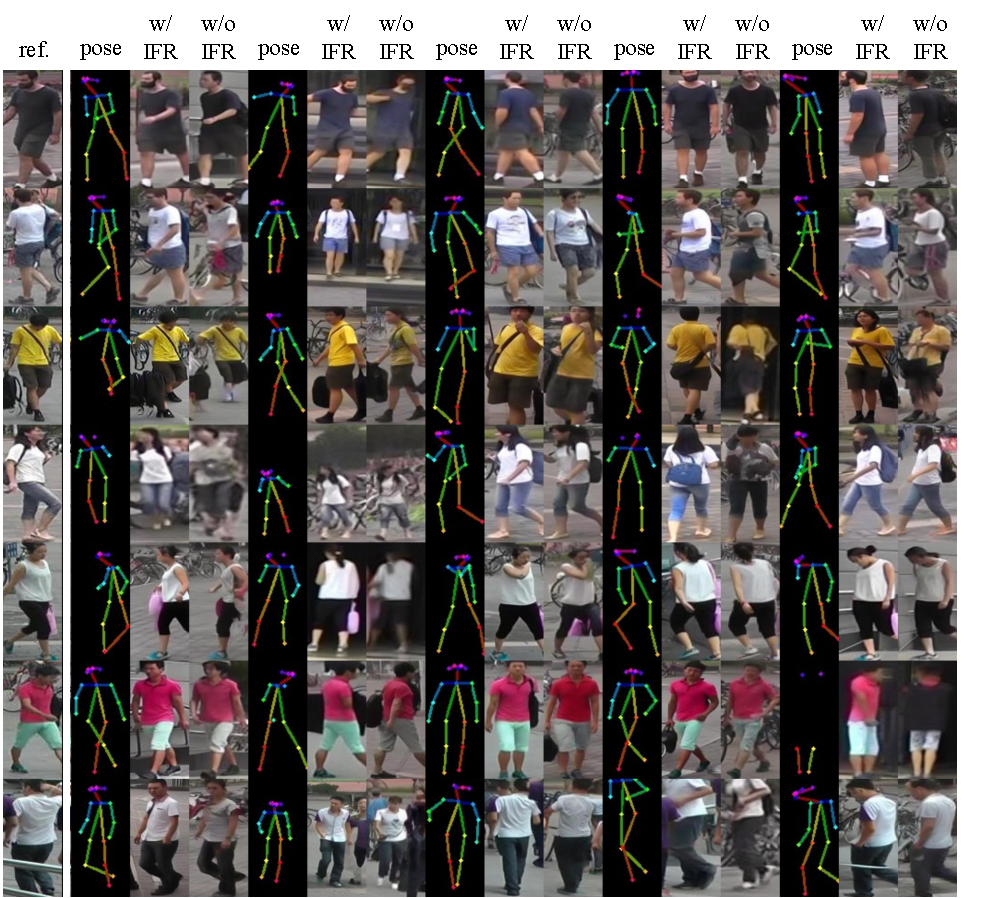
\includegraphics[width=0.95\linewidth]{figs/pdf/IFR.pdf}
\caption{The effects with and without the IFR module were visualized with five different poses randomly selected for each reference picture.}
\label{fig:IFR}
\end{figure}

\begin{table}
\small
    \centering
    \renewcommand{\arraystretch}{1}
    \renewcommand\tabcolsep{2pt}
    \begin{tabular}{c|ccc|ccc|ccc}
        \hline
        \multirow{2}{*}{\textbf{N}} & \multicolumn{3}{c|}{$\text{Gallery}^\text{IPG}$} & \multicolumn{3}{c|}{$\text{Query}^\text{IPG}$} & \multicolumn{3}{c}{$\text{Gallery}^\text{IPG}$+$\text{Query}^\text{IPG}$} \\ \cline{2-10}
          & mAP$\uparrow$ & R1$\uparrow$ & $\text{ID}^2$$\downarrow$ & mAP$\uparrow$ & R1$\uparrow$ & $\text{ID}^2$$\downarrow$ & mAP$\uparrow$ & R1$\uparrow$ & $\text{ID}^2$$\downarrow$ \\ \hline
        0 & 79.88 & 91.48 & 0.2313 & 79.88 & 91.48 & 0.1623 & 79.88 & 91.48 & 0.2193 \\
        1 & 80.96 & 90.97 & 0.2087 & 79.99 & 90.83 & 0.1363 & 82.13 & 92.01 & 0.1961 \\
        2 & 82.86 & 91.45 & 0.1904 & 81.17 & 92.04 & 0.1156 & 85.27 & 93.71 & 0.1773 \\
        3 & 83.42 & 91.75 & 0.1837 & 81.55 & 92.25 & 0.1077 & 86.16 & 94.21 & 0.1704 \\
        4 & 83.81 & 92.1  & 0.1795 & 81.76 & 92.34 & 0.1027 & 86.75 & 94.24 & 0.1661 \\
        5 & 84.07 & 91.83 & 0.1758 & 81.85 & 92.07 & 0.0984 & 87.23 & 94.71 & 0.1623 \\
        6 & 84.3  & 91.98 & 0.1730 & 81.96 & 92.52 & 0.0950 & 87.52 & 94.63 & 0.1593 \\
        7 & 84.49 & 91.86 & 0.1707 & 82.03 & 92.37 & 0.0922 & 87.76 & 94.60 & 0.1570 \\
        \rowcolor{gray!30}
        8 & 84.65 & 92.07 & 0.1691 & 82.18 & 92.40 & 0.0902 & 88.02 & 94.77 & 0.1553 \\ \hline
    \end{tabular}
    \caption{Performance Comparison by adding numbers of generated images for each image on gallery, query, and both}
    \label{tab:num}
\end{table}

\subsection{Abilation Study}
\textbf{Impact of the NFC and IPG.}
We conducted comprehensive ablation experiments on Neighbor Feature Centralization (NFC) and Feature ID-Centralizing through Identity-Guided Generation (IPG) methods. As shown in Table\ref{tab:ablation_fe_pg},\ref{tab:as_fe},\ref{tab:as_gen}, which show great improvements.
\begin{figure*}
\centering
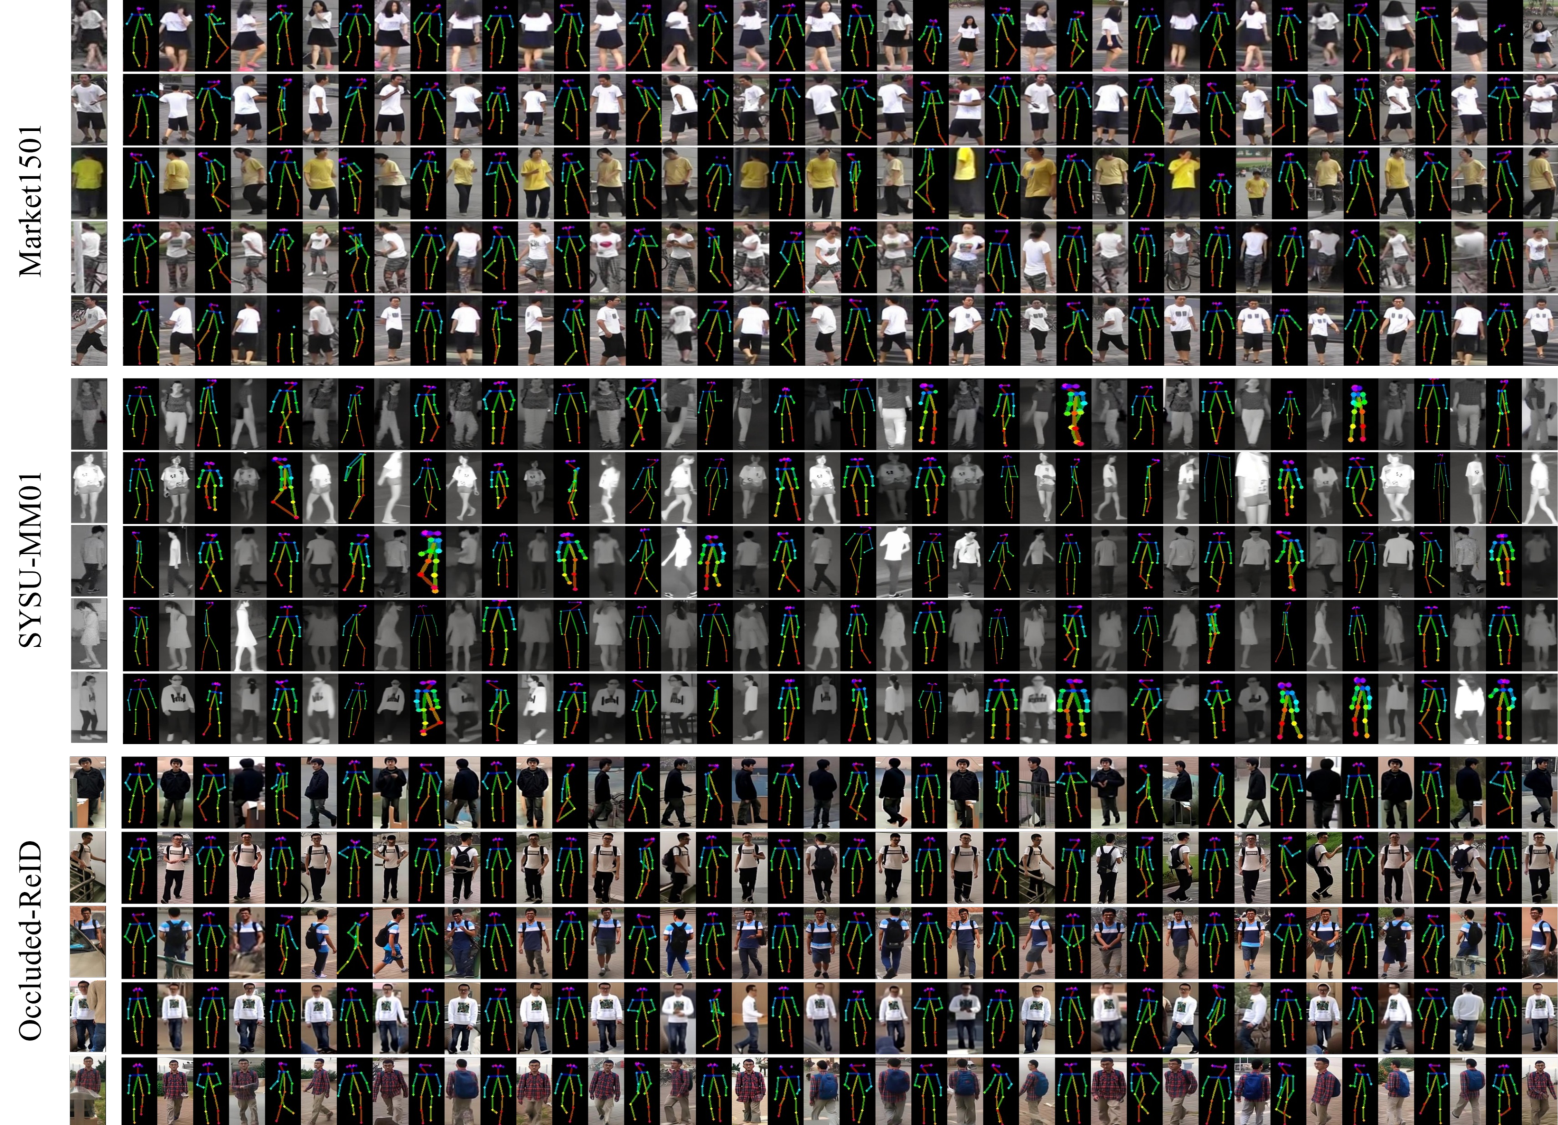
\includegraphics[width=\linewidth]{figs/pdf/random_sub_png.pdf}
\caption{Images generated with random poses. More randomly generated images can be found in Supplementary.}
\label{fig:randompose}
\end{figure*}
\\
\textbf{Effect of Feature Re-Distribute Module.}
We randomly selected 7 images from the Market1501 dataset, choosing 5 different poses for each image. We visualized the results both with and without Identity Feature Redistribute (IFR) Module. As shown in Fig.\ref{fig:IFR}, the impact of ID features on the generated outcomes is evident.
\\
\textbf{Effect of numbers of generated images.}
We randomly selected different numbers of images generated from the 8 representative poses to verify the effect of feature enhancement. As shown in Tab.\ref{tab:num}, the experimental results align with the theory mentioned in Section\ref{Feature Distribution}: the more features of the same ID that are aggregated, the more the adjustment noise extracted from individual images is reduced, enhancing the ID representation capability and resulting in improved matching performance.



\subsection{Visualizations}

\textbf{Different people with the same poses across datasets.}
We are working on Market1501, SYSU-MM01, and
Occluded-ReID datasets to visualize the 8 representative poses with only one model and results are shown in Fig.\ref{fig:intro}.
\\
\textbf{Random people with random poses.} To demonstrate the advancement of our model, as shown in Fig.\ref{fig:randompose}, we randomly chose samples from the whole dataset, and each sample randomly chose poses, including some problematic poses, fully demonstrating the diversity of model. \textbf{More examples on three datasets are visualized in }\textbf{Supplementary}.


% \subsection{Analysis on quality coefficient $\eta$ of Generation Model}

% Fig.\ref{fig:eta} illustrates the effect of adjusting the coefficient $\eta$ on the performance of the ReID model. To evaluate this impact, we gradually increased the value of $\eta$ and observed the changes in model performance on the mAP and Rank-1 metrics. 

% As the value of $\eta$ increases, the performance of the ReID model improves, reaching an optimal point. At $\eta = 2$, both mAP and Rank-1 achieve their maximum values of 88.02\% and 94.77\%, respectively. However, further increasing $\eta$ beyond this point leads to a slight decline in performance. It is easy to find that using generated images to centralize features is effective. However, considering the quality of the generated image, direct adding, although also effective, may not always achieve the best results. Therefore adjusting $\eta$ according to the generation quality of the model in this dataset can better centralize the features.
% \begin{figure}
% \centering
% 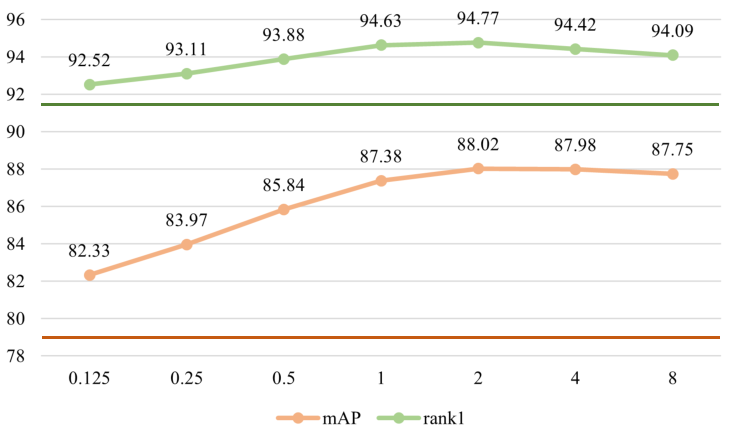
\includegraphics[width=0.9\linewidth]{figs/pdf/eta.pdf}
% \caption{Impact of the quality coefficient \( \eta \) with TransReID on Market1501. The dark color lines are the baseline.}
% \label{fig:eta}
% \end{figure}

\section{Conclusion and Discussion}~\label{sec:conclusion and discussion}
\vspace{-5pt}
\section{Conclusion}
\vspace{-5pt}
\label{sec:conclusion}

Room reidentification is a challenging yet crucial research area, with growing applications in fields like augmented reality and homecare robotics. In this paper, we introduce AirRoom, a training-free, object-aware approach for room reidentification. AirRoom leverages multi-level object-oriented features to capture both spatial and contextual information of indoor rooms. To evaluate AirRoom, we constructed four novel datasets specifically for room reidentification. Experimental results demonstrate its robustness to viewpoint variations and superior performance over state-of-the-art methods across nearly all metrics and datasets. Furthermore, the pipeline is highly flexible, maintaining high performance without relying on specific model configurations. Collectively, our work establishes AirRoom as a powerful and versatile solution for precise room reidentification, with broad potential for real-world applications.

\begin{center}
\textbf{Acknowledgments}  
\end{center}
% This work was partially supported by the DARPA grant DARPA-PS-23-13. The views and conclusions contained in this document are those of the authors and should not be interpreted as representing the official policies, either expressed or implied, of DARPA.
\begin{sloppypar}
\noindent This work was supported by the DARPA award HR00112490426. Any opinions, findings, conclusions, or recommendations expressed in this paper are those of the authors and do not necessarily reflect the views of DARPA.
\end{sloppypar}




{
\small
\begin{thebibliography}{10}

\bibitem{MipNeRF2021ICCV}
Jonathan~T Barron, Ben Mildenhall, Matthew Tancik, Peter Hedman, Ricardo Martin-Brualla, and Pratul~P Srinivasan.
\newblock Mip-nerf: A multiscale representation for anti-aliasing neural radiance fields.
\newblock In {\em ICCV}, pages 5855--5864, 2021.

\bibitem{cai2022pix2nerf}
Shengqu Cai, Anton Obukhov, Dengxin Dai, and Luc Van~Gool.
\newblock Pix2nerf: Unsupervised conditional p-gan for single image to neural radiance fields translation.
\newblock In {\em CVPR}, pages 3981--3990, 2022.

\bibitem{chan2021pi}
Eric~R Chan, Marco Monteiro, Petr Kellnhofer, Jiajun Wu, and Gordon Wetzstein.
\newblock pi-gan: Periodic implicit generative adversarial networks for 3d-aware image synthesis.
\newblock In {\em CVPR}, pages 5799--5809, 2021.

\bibitem{pixelSplat2023arXiv}
David Charatan, Sizhe Li, Andrea Tagliasacchi, and Vincent Sitzmann.
\newblock pixelsplat: 3d gaussian splats from image pairs for scalable generalizable 3d reconstruction.
\newblock {\em arXiv preprint arXiv:2312.12337}, 2023.

\bibitem{chen2021mvsnerf}
Anpei Chen, Zexiang Xu, Fuqiang Zhao, Xiaoshuai Zhang, Fanbo Xiang, Jingyi Yu, and Hao Su.
\newblock Mvsnerf: Fast generalizable radiance field reconstruction from multi-view stereo.
\newblock In {\em ICCV}, pages 14124--14133, 2021.

\bibitem{MVSplat2024arXiv}
Yuedong Chen, Haofei Xu, Chuanxia Zheng, Bohan Zhuang, Marc Pollefeys, Andreas Geiger, Tat-Jen Cham, and Jianfei Cai.
\newblock Mvsplat: Efficient 3d gaussian splatting from sparse multi-view images.
\newblock {\em arXiv preprint arXiv:2403.14627}, 2024.

\bibitem{du2021neural}
Yilun Du, Yinan Zhang, Hong-Xing Yu, Joshua~B Tenenbaum, and Jiajun Wu.
\newblock Neural radiance flow for 4d view synthesis and video processing.
\newblock In {\em ICCV}, pages 14304--14314. IEEE Computer Society, 2021.

\bibitem{duisterhof2023md}
Bardienus~P Duisterhof, Zhao Mandi, Yunchao Yao, Jia-Wei Liu, Mike~Zheng Shou, Shuran Song, and Jeffrey Ichnowski.
\newblock Md-splatting: Learning metric deformation from 4d gaussians in highly deformable scenes.
\newblock {\em arXiv preprint arXiv:2312.00583}, 2023.

\bibitem{fan2023lightgaussian}
Zhiwen Fan, Kevin Wang, Kairun Wen, Zehao Zhu, Dejia Xu, and Zhangyang Wang.
\newblock Lightgaussian: Unbounded 3d gaussian compression with 15x reduction and 200+ fps.
\newblock {\em arXiv preprint arXiv:2311.17245}, 2023.

\bibitem{Plenoxels2022CVPR}
Sara Fridovich-Keil, Alex Yu, Matthew Tancik, Qinhong Chen, Benjamin Recht, and Angjoo Kanazawa.
\newblock Plenoxels: Radiance fields without neural networks.
\newblock In {\em CVPR}, pages 5501--5510, 2022.

\bibitem{gao2023relightable}
Jian Gao, Chun Gu, Youtian Lin, Hao Zhu, Xun Cao, Li~Zhang, and Yao Yao.
\newblock Relightable 3d gaussian: Real-time point cloud relighting with brdf decomposition and ray tracing.
\newblock {\em arXiv preprint arXiv:2311.16043}, 2023.

\bibitem{FastNeRF2021ICCV}
Stephan~J Garbin, Marek Kowalski, Matthew Johnson, Jamie Shotton, and Julien Valentin.
\newblock Fastnerf: High-fidelity neural rendering at 200fps.
\newblock In {\em ICCV}, pages 14346--14355, 2021.

\bibitem{girish2023eagles}
Sharath Girish, Kamal Gupta, and Abhinav Shrivastava.
\newblock Eagles: Efficient accelerated 3d gaussians with lightweight encodings.
\newblock {\em arXiv preprint arXiv:2312.04564}, 2023.

\bibitem{gu2021stylenerf}
Jiatao Gu, Lingjie Liu, Peng Wang, and Christian Theobalt.
\newblock Stylenerf: A style-based 3d-aware generator for high-resolution image synthesis.
\newblock {\em arXiv preprint arXiv:2110.08985}, 2021.

\bibitem{EfficientNeRF2022CVPR}
Tao Hu, Shu Liu, Yilun Chen, Tiancheng Shen, and Jiaya Jia.
\newblock Efficientnerf efficient neural radiance fields.
\newblock In {\em CVPR}, pages 12902--12911, 2022.

\bibitem{jang2021codenerf}
Wonbong Jang and Lourdes Agapito.
\newblock Codenerf: Disentangled neural radiance fields for object categories.
\newblock In {\em ICCV}, pages 12949--12958, 2021.

\bibitem{jiang2023gaussianshader}
Yingwenqi Jiang, Jiadong Tu, Yuan Liu, Xifeng Gao, Xiaoxiao Long, Wenping Wang, and Yuexin Ma.
\newblock Gaussianshader: 3d gaussian splatting with shading functions for reflective surfaces.
\newblock {\em arXiv preprint arXiv:2311.17977}, 2023.

\bibitem{katsumata2023efficient}
Kai Katsumata, Duc~Minh Vo, and Hideki Nakayama.
\newblock An efficient 3d gaussian representation for monocular/multi-view dynamic scenes.
\newblock {\em arXiv preprint arXiv:2311.12897}, 2023.

\bibitem{3DGS2023ToG}
Bernhard Kerbl, Georgios Kopanas, Thomas Leimk{\"u}hler, and George Drettakis.
\newblock 3d gaussian splatting for real-time radiance field rendering.
\newblock {\em ToG}, 42(4):1--14, 2023.

\bibitem{li2021neural}
Zhengqi Li, Simon Niklaus, Noah Snavely, and Oliver Wang.
\newblock Neural scene flow fields for space-time view synthesis of dynamic scenes.
\newblock In {\em CVPR}, pages 6498--6508, 2021.

\bibitem{li2023dynibar}
Zhengqi Li, Qianqian Wang, Forrester Cole, Richard Tucker, and Noah Snavely.
\newblock Dynibar: Neural dynamic image-based rendering.
\newblock In {\em CVPR}, pages 4273--4284, 2023.

\bibitem{liang2023gs}
Zhihao Liang, Qi~Zhang, Ying Feng, Ying Shan, and Kui Jia.
\newblock Gs-ir: 3d gaussian splatting for inverse rendering.
\newblock {\em arXiv preprint arXiv:2311.16473}, 2023.

\bibitem{ENeRF2022SIGGRAPH}
Haotong Lin, Sida Peng, Zhen Xu, Yunzhi Yan, Qing Shuai, Hujun Bao, and Xiaowei Zhou.
\newblock Efficient neural radiance fields for interactive free-viewpoint video.
\newblock In {\em SIGGRAPH Asia}, pages 1--9, 2022.

\bibitem{ACID2021ICCV}
Andrew Liu, Richard Tucker, Varun Jampani, Ameesh Makadia, Noah Snavely, and Angjoo Kanazawa.
\newblock Infinite nature: Perpetual view generation of natural scenes from a single image.
\newblock In {\em ICCV}, pages 14458--14467, 2021.

\bibitem{liu2023semantic}
Fangfu Liu, Chubin Zhang, Yu~Zheng, and Yueqi Duan.
\newblock Semantic ray: Learning a generalizable semantic field with cross-reprojection attention.
\newblock In {\em CVPR}, pages 17386--17396, 2023.

\bibitem{NSVF2020NIPS}
Lingjie Liu, Jiatao Gu, Kyaw Zaw~Lin, Tat-Seng Chua, and Christian Theobalt.
\newblock Neural sparse voxel fields.
\newblock {\em NeurIPS}, 33:15651--15663, 2020.

\bibitem{lu2023scaffold}
Tao Lu, Mulin Yu, Linning Xu, Yuanbo Xiangli, Limin Wang, Dahua Lin, and Bo~Dai.
\newblock Scaffold-gs: Structured 3d gaussians for view-adaptive rendering.
\newblock {\em arXiv preprint arXiv:2312.00109}, 2023.

\bibitem{Dynamic3DGS2023arXiv}
Jonathon Luiten, Georgios Kopanas, Bastian Leibe, and Deva Ramanan.
\newblock Dynamic 3d gaussians: Tracking by persistent dynamic view synthesis.
\newblock {\em arXiv preprint arXiv:2308.09713}, 2023.

\bibitem{OccNet2019CVPR}
Lars Mescheder, Michael Oechsle, Michael Niemeyer, Sebastian Nowozin, and Andreas Geiger.
\newblock Occupancy networks: Learning 3d reconstruction in function space.
\newblock In {\em CVPR}, pages 4460--4470, 2019.

\bibitem{NeRF2021ACM}
Ben Mildenhall, Pratul~P Srinivasan, Matthew Tancik, Jonathan~T Barron, Ravi Ramamoorthi, and Ren Ng.
\newblock Nerf: Representing scenes as neural radiance fields for view synthesis.
\newblock {\em Communications of the ACM}, 65(1):99--106, 2021.

\bibitem{InstantNGP2022TOG}
Thomas M{\"u}ller, Alex Evans, Christoph Schied, and Alexander Keller.
\newblock Instant neural graphics primitives with a multiresolution hash encoding.
\newblock {\em ToG}, 41(4):1--15, 2022.

\bibitem{navaneet2023compact3d}
KL~Navaneet, Kossar~Pourahmadi Meibodi, Soroush~Abbasi Koohpayegani, and Hamed Pirsiavash.
\newblock Compact3d: Compressing gaussian splat radiance field models with vector quantization.
\newblock {\em arXiv preprint arXiv:2311.18159}, 2023.

\bibitem{niemeyer2022regnerf}
Michael Niemeyer, Jonathan~T Barron, Ben Mildenhall, Mehdi~SM Sajjadi, Andreas Geiger, and Noha Radwan.
\newblock Regnerf: Regularizing neural radiance fields for view synthesis from sparse inputs.
\newblock In {\em CVPR}, pages 5480--5490, 2022.

\bibitem{niemeyer2021giraffe}
Michael Niemeyer and Andreas Geiger.
\newblock Giraffe: Representing scenes as compositional generative neural feature fields.
\newblock In {\em CVPR}, pages 11453--11464, 2021.

\bibitem{DeepSDF2019CVPR}
Jeong~Joon Park, Peter Florence, Julian Straub, Richard Newcombe, and Steven Lovegrove.
\newblock Deepsdf: Learning continuous signed distance functions for shape representation.
\newblock In {\em CVPR}, pages 165--174, 2019.

\bibitem{pumarola2021d}
Albert Pumarola, Enric Corona, Gerard Pons-Moll, and Francesc Moreno-Noguer.
\newblock D-nerf: Neural radiance fields for dynamic scenes.
\newblock In {\em CVPR}, pages 10318--10327, 2021.

\bibitem{KiloNeRF2021ICCV}
Christian Reiser, Songyou Peng, Yiyi Liao, and Andreas Geiger.
\newblock Kilonerf: Speeding up neural radiance fields with thousands of tiny mlps.
\newblock In {\em ICCV}, pages 14335--14345, 2021.

\bibitem{schwarz2020graf}
Katja Schwarz, Yiyi Liao, Michael Niemeyer, and Andreas Geiger.
\newblock Graf: Generative radiance fields for 3d-aware image synthesis.
\newblock {\em NeurIPS}, 33:20154--20166, 2020.

\bibitem{LFN2021NIPS}
Vincent Sitzmann, Semon Rezchikov, William~T. Freeman, Joshua~B. Tenenbaum, and Fr{\'e}do Durand.
\newblock Light field networks: Neural scene representations with single-evaluation rendering.
\newblock In {\em NeurIPS}, 2021.

\bibitem{SRN2019NIPS}
Vincent Sitzmann, Michael Zollhofer, and Gordon Wetzstein.
\newblock Scene representation networks: Continuous 3d-structure-aware neural scene representations.
\newblock {\em NeurIPS}, 32, 2019.

\bibitem{SplatterImage2023arXiv}
Stanislaw Szymanowicz, Christian Rupprecht, and Andrea Vedaldi.
\newblock Splatter image: Ultra-fast single-view 3d reconstruction.
\newblock {\em arXiv preprint arXiv:2312.13150}, 2023.

\bibitem{BlockNeRF2022CVPR}
Matthew Tancik, Vincent Casser, Xinchen Yan, Sabeek Pradhan, Ben Mildenhall, Pratul~P Srinivasan, Jonathan~T Barron, and Henrik Kretzschmar.
\newblock Block-nerf: Scalable large scene neural view synthesis.
\newblock In {\em CVPR}, pages 8248--8258, 2022.

\bibitem{tian2023mononerf}
Fengrui Tian, Shaoyi Du, and Yueqi Duan.
\newblock Mononerf: Learning a generalizable dynamic radiance field from monocular videos.
\newblock In {\em ICCV}, pages 17903--17913, 2023.

\bibitem{tretschk2021non}
Edgar Tretschk, Ayush Tewari, Vladislav Golyanik, Michael Zollh{\"o}fer, Christoph Lassner, and Christian Theobalt.
\newblock Non-rigid neural radiance fields: Reconstruction and novel view synthesis of a dynamic scene from monocular video.
\newblock In {\em ICCV}, pages 12959--12970, 2021.

\bibitem{truong2023sparf}
Prune Truong, Marie-Julie Rakotosaona, Fabian Manhardt, and Federico Tombari.
\newblock Sparf: Neural radiance fields from sparse and noisy poses. ieee.
\newblock In {\em CVPR}, volume~1, 2023.

\bibitem{MegaNeRF2022CVPR}
Haithem Turki, Deva Ramanan, and Mahadev Satyanarayanan.
\newblock Mega-nerf: Scalable construction of large-scale nerfs for virtual fly-throughs.
\newblock In {\em CVPR}, pages 12922--12931, 2022.

\bibitem{SUDS2023CVPR}
Haithem Turki, Jason~Y Zhang, Francesco Ferroni, and Deva Ramanan.
\newblock Suds: Scalable urban dynamic scenes.
\newblock In {\em CVPR}, pages 12375--12385, 2023.

\bibitem{Fourierplenoctree2022CVPR}
Liao Wang, Jiakai Zhang, Xinhang Liu, Fuqiang Zhao, Yanshun Zhang, Yingliang Zhang, Minye Wu, Jingyi Yu, and Lan Xu.
\newblock Fourier plenoctrees for dynamic radiance field rendering in real-time.
\newblock In {\em CVPR}, pages 13524--13534, 2022.

\bibitem{wu20234d}
Guanjun Wu, Taoran Yi, Jiemin Fang, Lingxi Xie, Xiaopeng Zhang, Wei Wei, Wenyu Liu, Qi~Tian, and Xinggang Wang.
\newblock 4d gaussian splatting for real-time dynamic scene rendering.
\newblock {\em arXiv preprint arXiv:2310.08528}, 2023.

\bibitem{wynn2023diffusionerf}
Jamie Wynn and Daniyar Turmukhambetov.
\newblock Diffusionerf: Regularizing neural radiance fields with denoising diffusion models.
\newblock In {\em CVPR}, pages 4180--4189, 2023.

\bibitem{xian2021space}
Wenqi Xian, Jia-Bin Huang, Johannes Kopf, and Changil Kim.
\newblock Space-time neural irradiance fields for free-viewpoint video.
\newblock In {\em CVPR}, pages 9421--9431, 2021.

\bibitem{BungeeNeRF2022ECCV}
Yuanbo Xiangli, Linning Xu, Xingang Pan, Nanxuan Zhao, Anyi Rao, Christian Theobalt, Bo~Dai, and Dahua Lin.
\newblock Bungeenerf: Progressive neural radiance field for extreme multi-scale scene rendering.
\newblock In {\em ECCV}, pages 106--122. Springer, 2022.

\bibitem{xie2023physgaussian}
Tianyi Xie, Zeshun Zong, Yuxin Qiu, Xuan Li, Yutao Feng, Yin Yang, and Chenfanfu Jiang.
\newblock Physgaussian: Physics-integrated 3d gaussians for generative dynamics.
\newblock {\em arXiv preprint arXiv:2311.12198}, 2023.

\bibitem{xiong2023sparsegs}
Haolin Xiong, Sairisheek Muttukuru, Rishi Upadhyay, Pradyumna Chari, and Achuta Kadambi.
\newblock Sparsegs: Real-time 360 $\{$$\backslash$deg$\}$ sparse view synthesis using gaussian splatting.
\newblock {\em arXiv preprint arXiv:2312.00206}, 2023.

\bibitem{xu2023murf}
Haofei Xu, Anpei Chen, Yuedong Chen, Christos Sakaridis, Yulun Zhang, Marc Pollefeys, Andreas Geiger, and Fisher Yu.
\newblock Murf: Multi-baseline radiance fields.
\newblock {\em arXiv preprint arXiv:2312.04565}, 2023.

\bibitem{GridNeRF2023CVPR}
Linning Xu, Yuanbo Xiangli, Sida Peng, Xingang Pan, Nanxuan Zhao, Christian Theobalt, Bo~Dai, and Dahua Lin.
\newblock Grid-guided neural radiance fields for large urban scenes.
\newblock In {\em CVPR}, pages 8296--8306, 2023.

\bibitem{yan2023multi}
Zhiwen Yan, Weng~Fei Low, Yu~Chen, and Gim~Hee Lee.
\newblock Multi-scale 3d gaussian splatting for anti-aliased rendering.
\newblock {\em arXiv preprint arXiv:2311.17089}, 2023.

\bibitem{yang2023real}
Zeyu Yang, Hongye Yang, Zijie Pan, Xiatian Zhu, and Li~Zhang.
\newblock Real-time photorealistic dynamic scene representation and rendering with 4d gaussian splatting.
\newblock {\em arXiv preprint arXiv:2310.10642}, 2023.

\bibitem{DGA2020NIPS}
Lior Yariv, Yoni Kasten, Dror Moran, Meirav Galun, Matan Atzmon, Basri Ronen, and Yaron Lipman.
\newblock Multiview neural surface reconstruction by disentangling geometry and appearance.
\newblock {\em NeurIPS}, 33:2492--2502, 2020.

\bibitem{PlenOctree2021CVPR}
Alex Yu, Ruilong Li, Matthew Tancik, Hao Li, Ren Ng, and Angjoo Kanazawa.
\newblock Plenoctrees for real-time rendering of neural radiance fields.
\newblock In {\em ICCV}, pages 5752--5761, 2021.

\bibitem{pixelNeRF2021CVPR}
Alex Yu, Vickie Ye, Matthew Tancik, and Angjoo Kanazawa.
\newblock pixelnerf: Neural radiance fields from one or few images.
\newblock In {\em CVPR}, pages 4578--4587, 2021.

\bibitem{LPIPS2018CVPR}
Richard Zhang, Phillip Isola, Alexei~A Efros, Eli Shechtman, and Oliver Wang.
\newblock The unreasonable effectiveness of deep features as a perceptual metric.
\newblock In {\em CVPR}, pages 586--595, 2018.

\bibitem{GPSGaussian2023arXiv}
Shunyuan Zheng, Boyao Zhou, Ruizhi Shao, Boning Liu, Shengping Zhang, Liqiang Nie, and Yebin Liu.
\newblock Gps-gaussian: Generalizable pixel-wise 3d gaussian splatting for real-time human novel view synthesis.
\newblock {\em arXiv preprint arXiv:2312.02155}, 2023.

\bibitem{RealEstate10K2018}
Tinghui Zhou, Richard Tucker, John Flynn, Graham Fyffe, and Noah Snavely.
\newblock Stereo magnification: Learning view synthesis using multiplane images.
\newblock {\em arXiv preprint arXiv:1805.09817}, 2018.

\bibitem{zhu2023fsgs}
Zehao Zhu, Zhiwen Fan, Yifan Jiang, and Zhangyang Wang.
\newblock Fsgs: Real-time few-shot view synthesis using gaussian splatting.
\newblock {\em arXiv preprint arXiv:2312.00451}, 2023.

\end{thebibliography}


  % \bibliographystyle{plain}
  % \bibliography{main}
}


% \newpage
% \appendix
% \input{sec/X_supplementary}

% \input{rebuttal}

% \clearpage
% \newpage
% \section*{NeurIPS Paper Checklist}
% 
%%%%%%%%%%%%%%%%%%%%%%%%%%%%%%%%%%%%%%%%%%%%%%%%%%%%%%%%%%%%

\newpage
\section*{NeurIPS Paper Checklist}
\begin{enumerate}

\item {\bf Claims}
    \item[] Question: Do the main claims made in the abstract and introduction accurately reflect the paper's contributions and scope?
    \item[] Answer: \answerYes{} % Replace by \answerYes{}, \answerNo{}, or \answerNA{}.
    \item[] Justification: We make claims in Abstract and Introduction (Sec. \ref{introduction}), which match results in Experiments (Sec. \ref{experiments}).
    \item[] Guidelines: 
    \begin{itemize}
        \item The answer NA means that the abstract and introduction do not include the claims made in the paper.
        \item The abstract and/or introduction should clearly state the claims made, including the contributions made in the paper and important assumptions and limitations. A No or NA answer to this question will not be perceived well by the reviewers. 
        \item The claims made should match theoretical and experimental results, and reflect how much the results can be expected to generalize to other settings. 
        \item It is fine to include aspirational goals as motivation as long as it is clear that these goals are not attained by the paper. 
    \end{itemize}

\item {\bf Limitations}
    \item[] Question: Does the paper discuss the limitations of the work performed by the authors?
    \item[] Answer: \answerYes{} % Replace by \answerYes{}, \answerNo{}, or \answerNA{}.
    \item[] Justification: We discuss limitations in Conclusion (Sec. \ref{conclusion}).
    \item[] Guidelines:
    \begin{itemize}
        \item The answer NA means that the paper has no limitation while the answer No means that the paper has limitations, but those are not discussed in the paper. 
        \item The authors are encouraged to create a separate "Limitations" section in their paper.
        \item The paper should point out any strong assumptions and how robust the results are to violations of these assumptions (e.g., independence assumptions, noiseless settings, model well-specification, asymptotic approximations only holding locally). The authors should reflect on how these assumptions might be violated in practice and what the implications would be.
        \item The authors should reflect on the scope of the claims made, e.g., if the approach was only tested on a few datasets or with a few runs. In general, empirical results often depend on implicit assumptions, which should be articulated.
        \item The authors should reflect on the factors that influence the performance of the approach. For example, a facial recognition algorithm may perform poorly when image resolution is low or images are taken in low lighting. Or a speech-to-text system might not be used reliably to provide closed captions for online lectures because it fails to handle technical jargon.
        \item The authors should discuss the computational efficiency of the proposed algorithms and how they scale with dataset size.
        \item If applicable, the authors should discuss possible limitations of their approach to address problems of privacy and fairness.
        \item While the authors might fear that complete honesty about limitations might be used by reviewers as grounds for rejection, a worse outcome might be that reviewers discover limitations that aren't acknowledged in the paper. The authors should use their best judgment and recognize that individual actions in favor of transparency play an important role in developing norms that preserve the integrity of the community. Reviewers will be specifically instructed to not penalize honesty concerning limitations.
    \end{itemize}

\item {\bf Theory Assumptions and Proofs}
    \item[] Question: For each theoretical result, does the paper provide the full set of assumptions and a complete (and correct) proof?
    \item[] Answer: \answerNA{} % Replace by \answerYes{}, \answerNo{}, or \answerNA{}.
    \item[] Justification: Our work does not include theoretical results.
    \item[] Guidelines:
    \begin{itemize}
        \item The answer NA means that the paper does not include theoretical results. 
        \item All the theorems, formulas, and proofs in the paper should be numbered and cross-referenced.
        \item All assumptions should be clearly stated or referenced in the statement of any theorems.
        \item The proofs can either appear in the main paper or the supplemental material, but if they appear in the supplemental material, the authors are encouraged to provide a short proof sketch to provide intuition. 
        \item Inversely, any informal proof provided in the core of the paper should be complemented by formal proofs provided in appendix or supplemental material.
        \item Theorems and Lemmas that the proof relies upon should be properly referenced. 
    \end{itemize}

    \item {\bf Experimental Result Reproducibility}
    \item[] Question: Does the paper fully disclose all the information needed to reproduce the main experimental results of the paper to the extent that it affects the main claims and/or conclusions of the paper (regardless of whether the code and data are provided or not)?
    \item[] Answer: \answerYes{} % Replace by \answerYes{}, \answerNo{}, or \answerNA{}.
    \item[] Justification: We provide the detailed information needed to reproduce our results in Appendix \ref{app:imp_detail}. We will also make our codes and model checkpoints available to public.
    \item[] Guidelines:
    \begin{itemize}
        \item The answer NA means that the paper does not include experiments.
        \item If the paper includes experiments, a No answer to this question will not be perceived well by the reviewers: Making the paper reproducible is important, regardless of whether the code and data are provided or not.
        \item If the contribution is a dataset and/or model, the authors should describe the steps taken to make their results reproducible or verifiable. 
        \item Depending on the contribution, reproducibility can be accomplished in various ways. For example, if the contribution is a novel architecture, describing the architecture fully might suffice, or if the contribution is a specific model and empirical evaluation, it may be necessary to either make it possible for others to replicate the model with the same dataset, or provide access to the model. In general. releasing code and data is often one good way to accomplish this, but reproducibility can also be provided via detailed instructions for how to replicate the results, access to a hosted model (e.g., in the case of a large language model), releasing of a model checkpoint, or other means that are appropriate to the research performed.
        \item While NeurIPS does not require releasing code, the conference does require all submissions to provide some reasonable avenue for reproducibility, which may depend on the nature of the contribution. For example
        \begin{enumerate}
            \item If the contribution is primarily a new algorithm, the paper should make it clear how to reproduce that algorithm.
            \item If the contribution is primarily a new model architecture, the paper should describe the architecture clearly and fully.
            \item If the contribution is a new model (e.g., a large language model), then there should either be a way to access this model for reproducing the results or a way to reproduce the model (e.g., with an open-source dataset or instructions for how to construct the dataset).
            \item We recognize that reproducibility may be tricky in some cases, in which case authors are welcome to describe the particular way they provide for reproducibility. In the case of closed-source models, it may be that access to the model is limited in some way (e.g., to registered users), but it should be possible for other researchers to have some path to reproducing or verifying the results.
        \end{enumerate}
    \end{itemize}


\item {\bf Open access to data and code}
    \item[] Question: Does the paper provide open access to the data and code, with sufficient instructions to faithfully reproduce the main experimental results, as described in supplemental material?
    \item[] Answer: \answerYes{} % Replace by \answerYes{}, \answerNo{}, or \answerNA{}.
    \item[] Justification: We submit codes as supplemental material and provide instructions for reproducing our results.
    \item[] Guidelines:
    \begin{itemize}
        \item The answer NA means that paper does not include experiments requiring code.
        \item Please see the NeurIPS code and data submission guidelines (\url{https://nips.cc/public/guides/CodeSubmissionPolicy}) for more details.
        \item While we encourage the release of code and data, we understand that this might not be possible, so “No” is an acceptable answer. Papers cannot be rejected simply for not including code, unless this is central to the contribution (e.g., for a new open-source benchmark).
        \item The instructions should contain the exact command and environment needed to run to reproduce the results. See the NeurIPS code and data submission guidelines (\url{https://nips.cc/public/guides/CodeSubmissionPolicy}) for more details.
        \item The authors should provide instructions on data access and preparation, including how to access the raw data, preprocessed data, intermediate data, and generated data, etc.
        \item The authors should provide scripts to reproduce all experimental results for the new proposed method and baselines. If only a subset of experiments are reproducible, they should state which ones are omitted from the script and why.
        \item At submission time, to preserve anonymity, the authors should release anonymized versions (if applicable).
        \item Providing as much information as possible in supplemental material (appended to the paper) is recommended, but including URLs to data and code is permitted.
    \end{itemize}


\item {\bf Experimental Setting/Details}
    \item[] Question: Does the paper specify all the training and test details (e.g., data splits, hyperparameters, how they were chosen, type of optimizer, etc.) necessary to understand the results?
    \item[] Answer: \answerYes{} % Replace by \answerYes{}, \answerNo{}, or \answerNA{}.
    \item[] Justification: We describe experimental setting/details in Appendix \ref{app:imp_detail}.
    \item[] Guidelines:
    \begin{itemize}
        \item The answer NA means that the paper does not include experiments.
        \item The experimental setting should be presented in the core of the paper to a level of detail that is necessary to appreciate the results and make sense of them.
        \item The full details can be provided either with the code, in appendix, or as supplemental material.
    \end{itemize}

\item {\bf Experiment Statistical Significance}
    \item[] Question: Does the paper report error bars suitably and correctly defined or other appropriate information about the statistical significance of the experiments?
    \item[] Answer: \answerNo{} % Replace by \answerYes{}, \answerNo{}, or \answerNA{}.
    \item[] Justification: Due to the limited compute resources, we cannot afford to run experiments several times to report error bars.
    \item[] Guidelines:
    \begin{itemize}
        \item The answer NA means that the paper does not include experiments.
        \item The authors should answer "Yes" if the results are accompanied by error bars, confidence intervals, or statistical significance tests, at least for the experiments that support the main claims of the paper.
        \item The factors of variability that the error bars are capturing should be clearly stated (for example, train/test split, initialization, random drawing of some parameter, or overall run with given experimental conditions).
        \item The method for calculating the error bars should be explained (closed form formula, call to a library function, bootstrap, etc.)
        \item The assumptions made should be given (e.g., Normally distributed errors).
        \item It should be clear whether the error bar is the standard deviation or the standard error of the mean.
        \item It is OK to report 1-sigma error bars, but one should state it. The authors should preferably report a 2-sigma error bar than state that they have a 96\% CI, if the hypothesis of Normality of errors is not verified.
        \item For asymmetric distributions, the authors should be careful not to show in tables or figures symmetric error bars that would yield results that are out of range (e.g. negative error rates).
        \item If error bars are reported in tables or plots, The authors should explain in the text how they were calculated and reference the corresponding figures or tables in the text.
    \end{itemize}

\item {\bf Experiments Compute Resources}
    \item[] Question: For each experiment, does the paper provide sufficient information on the computer resources (type of compute workers, memory, time of execution) needed to reproduce the experiments?
    \item[] Answer: \answerYes{} % Replace by \answerYes{}, \answerNo{}, or \answerNA{}.
    \item[] Justification: We describe the computer resources in Sec. \label{experiments}.
    \item[] Guidelines:
    \begin{itemize}
        \item The answer NA means that the paper does not include experiments.
        \item The paper should indicate the type of compute workers CPU or GPU, internal cluster, or cloud provider, including relevant memory and storage.
        \item The paper should provide the amount of compute required for each of the individual experimental runs as well as estimate the total compute. 
        \item The paper should disclose whether the full research project required more compute than the experiments reported in the paper (e.g., preliminary or failed experiments that didn't make it into the paper). 
    \end{itemize}
    
\item {\bf Code Of Ethics}
    \item[] Question: Does the research conducted in the paper conform, in every respect, with the NeurIPS Code of Ethics \url{https://neurips.cc/public/EthicsGuidelines}?
    \item[] Answer: \answerYes{} % Replace by \answerYes{}, \answerNo{}, or \answerNA{}.
    \item[] Justification: Our research conform with the NeurIPS Code of Ethics.
    \item[] Guidelines:
    \begin{itemize}
        \item The answer NA means that the authors have not reviewed the NeurIPS Code of Ethics.
        \item If the authors answer No, they should explain the special circumstances that require a deviation from the Code of Ethics.
        \item The authors should make sure to preserve anonymity (e.g., if there is a special consideration due to laws or regulations in their jurisdiction).
    \end{itemize}


\item {\bf Broader Impacts}
    \item[] Question: Does the paper discuss both potential positive societal impacts and negative societal impacts of the work performed?
    \item[] Answer: \answerYes{} % Replace by \answerYes{}, \answerNo{}, or \answerNA{}.
    \item[] Justification: We discuss about potential positive societal impacts in Conclusion (Sec. \ref{conclusion}).
    \item[] Guidelines:
    \begin{itemize}
        \item The answer NA means that there is no societal impact of the work performed.
        \item If the authors answer NA or No, they should explain why their work has no societal impact or why the paper does not address societal impact.
        \item Examples of negative societal impacts include potential malicious or unintended uses (e.g., disinformation, generating fake profiles, surveillance), fairness considerations (e.g., deployment of technologies that could make decisions that unfairly impact specific groups), privacy considerations, and security considerations.
        \item The conference expects that many papers will be foundational research and not tied to particular applications, let alone deployments. However, if there is a direct path to any negative applications, the authors should point it out. For example, it is legitimate to point out that an improvement in the quality of generative models could be used to generate deepfakes for disinformation. On the other hand, it is not needed to point out that a generic algorithm for optimizing neural networks could enable people to train models that generate Deepfakes faster.
        \item The authors should consider possible harms that could arise when the technology is being used as intended and functioning correctly, harms that could arise when the technology is being used as intended but gives incorrect results, and harms following from (intentional or unintentional) misuse of the technology.
        \item If there are negative societal impacts, the authors could also discuss possible mitigation strategies (e.g., gated release of models, providing defenses in addition to attacks, mechanisms for monitoring misuse, mechanisms to monitor how a system learns from feedback over time, improving the efficiency and accessibility of ML).
    \end{itemize}
    
\item {\bf Safeguards}
    \item[] Question: Does the paper describe safeguards that have been put in place for responsible release of data or models that have a high risk for misuse (e.g., pretrained language models, image generators, or scraped datasets)?
    \item[] Answer: \answerNA{} % Replace by \answerYes{}, \answerNo{}, or \answerNA{}.
    \item[] Justification: Our work poses no such risks.
    \item[] Guidelines:
    \begin{itemize}
        \item The answer NA means that the paper poses no such risks.
        \item Released models that have a high risk for misuse or dual-use should be released with necessary safeguards to allow for controlled use of the model, for example by requiring that users adhere to usage guidelines or restrictions to access the model or implementing safety filters. 
        \item Datasets that have been scraped from the Internet could pose safety risks. The authors should describe how they avoided releasing unsafe images.
        \item We recognize that providing effective safeguards is challenging, and many papers do not require this, but we encourage authors to take this into account and make a best faith effort.
    \end{itemize}

\item {\bf Licenses for existing assets}
    \item[] Question: Are the creators or original owners of assets (e.g., code, data, models), used in the paper, properly credited and are the license and terms of use explicitly mentioned and properly respected?
    \item[] Answer: \answerYes{} % Replace by \answerYes{}, \answerNo{}, or \answerNA{}.
    \item[] Justification: We cite the original paper in Sec. \ref{experiments}.
    \item[] Guidelines:
    \begin{itemize}
        \item The answer NA means that the paper does not use existing assets.
        \item The authors should cite the original paper that produced the code package or dataset.
        \item The authors should state which version of the asset is used and, if possible, include a URL.
        \item The name of the license (e.g., CC-BY 4.0) should be included for each asset.
        \item For scraped data from a particular source (e.g., website), the copyright and terms of service of that source should be provided.
        \item If assets are released, the license, copyright information, and terms of use in the package should be provided. For popular datasets, \url{paperswithcode.com/datasets} has curated licenses for some datasets. Their licensing guide can help determine the license of a dataset.
        \item For existing datasets that are re-packaged, both the original license and the license of the derived asset (if it has changed) should be provided.
        \item If this information is not available online, the authors are encouraged to reach out to the asset's creators.
    \end{itemize}

\item {\bf New Assets}
    \item[] Question: Are new assets introduced in the paper well documented and is the documentation provided alongside the assets?
    \item[] Answer: \answerYes{} % Replace by \answerYes{}, \answerNo{}, or \answerNA{}.
    \item[] Justification: We provide detailed instruction of codes in supplementary materials.
    \item[] Guidelines:
    \begin{itemize}
        \item The answer NA means that the paper does not release new assets.
        \item Researchers should communicate the details of the dataset/code/model as part of their submissions via structured templates. This includes details about training, license, limitations, etc. 
        \item The paper should discuss whether and how consent was obtained from people whose asset is used.
        \item At submission time, remember to anonymize your assets (if applicable). You can either create an anonymized URL or include an anonymized zip file.
    \end{itemize}

\item {\bf Crowdsourcing and Research with Human Subjects}
    \item[] Question: For crowdsourcing experiments and research with human subjects, does the paper include the full text of instructions given to participants and screenshots, if applicable, as well as details about compensation (if any)? 
    \item[] Answer: \answerNA{} % Replace by \answerYes{}, \answerNo{}, or \answerNA{}.
    \item[] Justification: Our work dose not involve crowdsourcing nor research with human subjects.
    \item[] Guidelines:
    \begin{itemize}
        \item The answer NA means that the paper does not involve crowdsourcing nor research with human subjects.
        \item Including this information in the supplemental material is fine, but if the main contribution of the paper involves human subjects, then as much detail as possible should be included in the main paper. 
        \item According to the NeurIPS Code of Ethics, workers involved in data collection, curation, or other labor should be paid at least the minimum wage in the country of the data collector. 
    \end{itemize}

\item {\bf Institutional Review Board (IRB) Approvals or Equivalent for Research with Human Subjects}
    \item[] Question: Does the paper describe potential risks incurred by study participants, whether such risks were disclosed to the subjects, and whether Institutional Review Board (IRB) approvals (or an equivalent approval/review based on the requirements of your country or institution) were obtained?
    \item[] Answer: \answerNA{} % Replace by \answerYes{}, \answerNo{}, or \answerNA{}.
    \item[] Justification: Our work dose not involve crowdsourcing nor research with human subjects.
    \item[] Guidelines:
    \begin{itemize}
        \item The answer NA means that the paper does not involve crowdsourcing nor research with human subjects.
        \item Depending on the country in which research is conducted, IRB approval (or equivalent) may be required for any human subjects research. If you obtained IRB approval, you should clearly state this in the paper. 
        \item We recognize that the procedures for this may vary significantly between institutions and locations, and we expect authors to adhere to the NeurIPS Code of Ethics and the guidelines for their institution. 
        \item For initial submissions, do not include any information that would break anonymity (if applicable), such as the institution conducting the review.
    \end{itemize}

\end{enumerate}






\end{document}